\documentclass[11pt]{beamer}
\usepackage[utf8]{inputenc}
\usepackage[T1]{fontenc}
\usepackage[spanish]{babel}
\newtheorem{teorema}[theorem]{Teorema}
\usepackage[color,matrix,arrow]{xy}
\usepackage{listings}
\usepackage{minipage-marginpar}
\usepackage{multicol}
\spanishdecimal{.}
\usepackage{ragged2e}
\usepackage{upquote} % Upright quotes for verbatim code
\usepackage{eurosym} % defines \euro

\theoremstyle{definition}
\newtheorem{defn}{Definici\'on}[Definition]
%\newtheorem{conj}{Conjecture}[section]
%\newtheorem{exmp}{Example}[section]
%###########################################################################33


%########################################################################3
%\newtheorem{definicion}[Definition]{Definicion}
\usetheme{EastLansing}


\date{21 de febrero de 2019}	% Insert the date of your presentation. \today gives an unsurprising automatic date.

\title[Parametrizaci\'on]{M\'etodo de parametrizaci\'on:\\Variedades estables e inestables en mapeos Hamiltonianos de dos dimensiones}
\author[E. \'Alvarez]{Evelyn \'Alvarez Cruz} % Insert your name

\institute[FC]{Facultad de Ciencias\\ Universidad Nacional Aut\'onoma de M\'exico} % Self-explanatory


\begin{document}
	%\author{}
	%\title{}
	%\subtitle{}
	%\logo{}
	%\institute{}
	%\date{}
	%\subject{}
	%\setbeamercovered{transparent}
	%\setbeamertemplate{navigation symbols}{}
	\begin{frame}[plain]
	\maketitle
\end{frame}
%--------------------------------------------------------------------------
\begin{frame}{Resumen}	
\begin{itemize}
	\item[1] Motivaciones.
	\item[2] El m\'etodo de parametrizaci\'on.
	\begin{itemize}
		\item[2.1] Ejemplo de aplicaci\'on al mapeo est\'andar. 
	\end{itemize}
	\item[3] Implementaci\'on
	\item[4] Ejemplos
	\begin{itemize}
		\item[4.1] El mapeo est\'andar
		\item[4.2] El mapeo de H\'enon
		\item[4.3] El mapeo exponencial
	\end{itemize}
	\item[5] Conclusiones y perspectivas
\end{itemize}

\end{frame}



%-----------------------------------------------------------------------





%----------------------------------------------------------------------------------------------------------
\begin{frame}{Motivaciones}	
\begin{itemize}
\item Los mapeos discretos pueden describir sistemas f\'isicos.\\
\begin{figure}
	\centering
	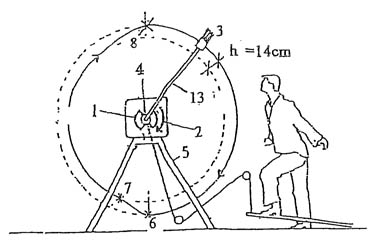
\includegraphics[scale=1.5]{kicked.jpg}
	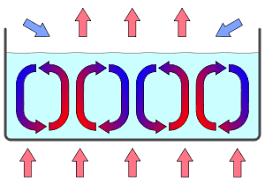
\includegraphics[scale=.4]{conveccion.png}
	\label{fig:rotor}
\end{figure}
\item Conocer la din\'amica alrededor de puntos fijos.\\

\item Conocer el comportamiento de las variedades estables e inestables asociadas a puntos fijos hiperb\'olicos.\\

\item Los m\'etodos mediante los cuales se calculan las variedades son iterativos.\\
\end{itemize}

\end{frame}
%------------------------------------------------------------------------------------------
\begin{frame}{M\'etodo de parametrizaci\'on}
Sea $\mathbf{f}:\mathbb{R}^{2}\rightarrow\mathbb{R}^{2}$ un mapeo Hamiltoniano, el cual tiene un punto fijo hiperb\'olico $\mathbf{x}_{*}$.\\
%\begin{teorema}[Hartman-Grobman]
%Sea $\mathbf{x}_{*}$ un punto fijo hiperb\'olico de $\mathbf{f}$ %y suponga que $\mathbf{f'}(\mathbf{x_{*}})=\lambda_{1}$ con $ %\vert \lambda_{1}\vert\neq 0,1 $. Entonces hay vecindades $U$ de %$\mathbf{x_{*}}$ y $V$ de $0\in\mathbb{R}$ y un homeomorfismo %$h:U\rightarrow\mathbb{R}$ que conjuga $\mathbf{f}$ en $U$ con %el mapeo lineal $L(\mathbf{x})=\lambda\mathbf{x}$  en $V$.
%\end{teorema}
Tomando la linealización:
\begin{equation}
\mathbf{x}_{n+1} =\mathbf{A}\mathbf{x}_{n}, \quad \mathbf{A}=D\mathbf{f}(\mathbf{x}_{*})
\label{sistema_lineal}
\end{equation}
donde \\
\begin{equation}
\vert \lambda_{1}\vert<1 \quad \rightarrow \mathbf{u}
\label{primer_valorp}
\end{equation}
\begin{equation}
\vert \lambda_{2}\vert>1 \quad \rightarrow \mathbf{v}
\label{segundo_valorp}
\end{equation}

\end{frame}
%----------------------------------------------------------------------
\begin{frame}
\begin{defn}[Variedad estable e inestable]
\begin{equation}
W^{s}=\lbrace \mathbf{x} : \mathbf{f}^{n}(\mathbf{x})\rightarrow \mathbf{x}_{*} \quad \mathrm{cuando} \quad n\rightarrow \infty \rbrace
\label{variedad estable}
\end{equation}

\begin{equation}
W^{u}=\lbrace \mathbf{x} : \mathbf{f}^{n}(\mathbf{x})\rightarrow \mathbf{x}_{*} \quad \mathrm{cuando} \quad n\rightarrow -\infty \rbrace.
\label{variedad inestable}
\end{equation}

\end{defn}

\begin{figure}
\centering
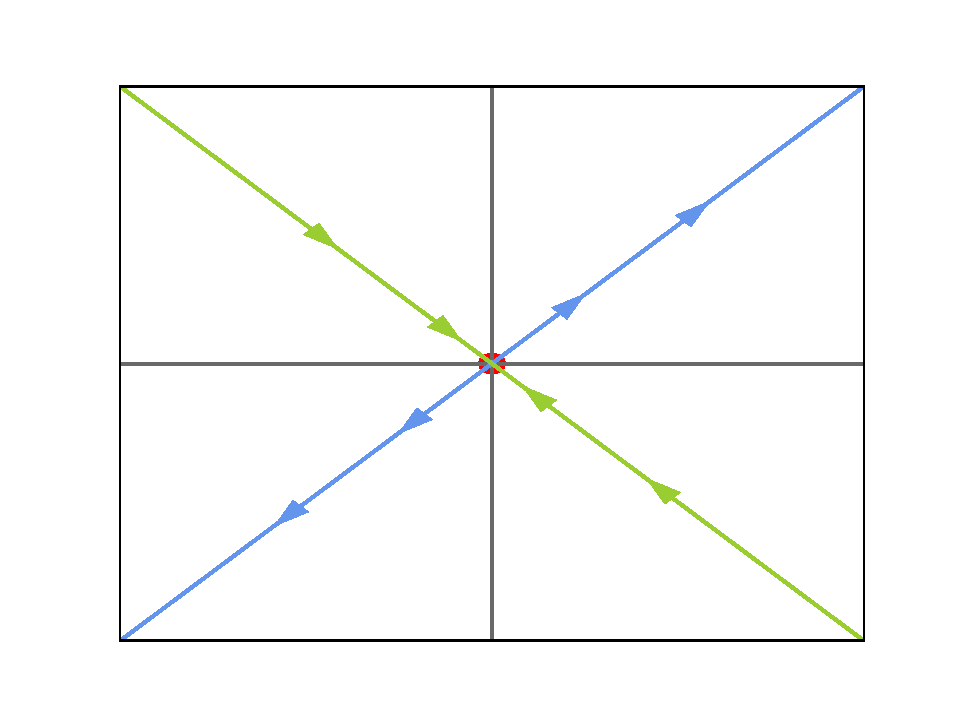
\includegraphics[scale=0.4]{hyperbolic2.pdf}
\caption{Punto fijo hiperb\'olico.}
\label{hiperbolico}
\end{figure}

\end{frame}
%----------------------------------------------------
\begin{frame}
%\begin{definition}[Conjunto invariante]
%\end{definition}
Sea  $\mathbf{I} \subset \mathbf{W}$ subconjunto de la variedad, para cualquier $\mathbf{x}_{i}\in  \mathbf{I}$  y $ n\in\mathbb{N}$ 
\begin{equation}
\mathbf{f}^{n}(\mathbf{x}_{i}) \in \mathbf{W}
\end{equation}
\begin{figure}
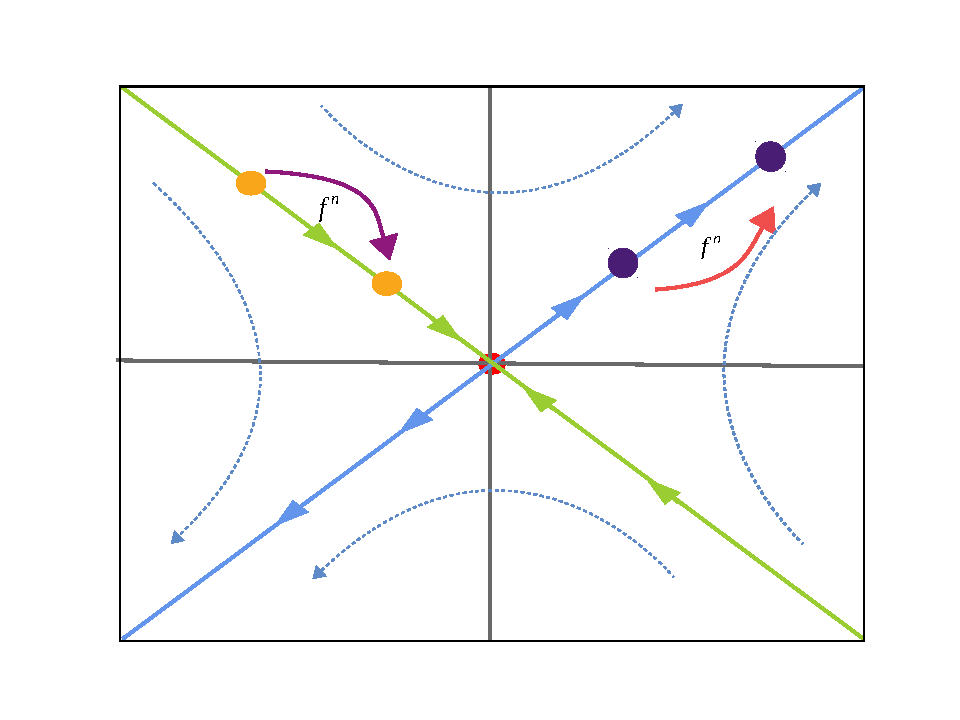
\includegraphics[scale=0.43]{hyperbolic2A.pdf}
\caption{Comportamiento de las variedades.}
\end{figure}
\end{frame}
%-------------------------------------------------------------
\begin{frame}
Para describir la variedad usamos una parametrizaci\'on $\mathcal{P}$.
\begin{figure}
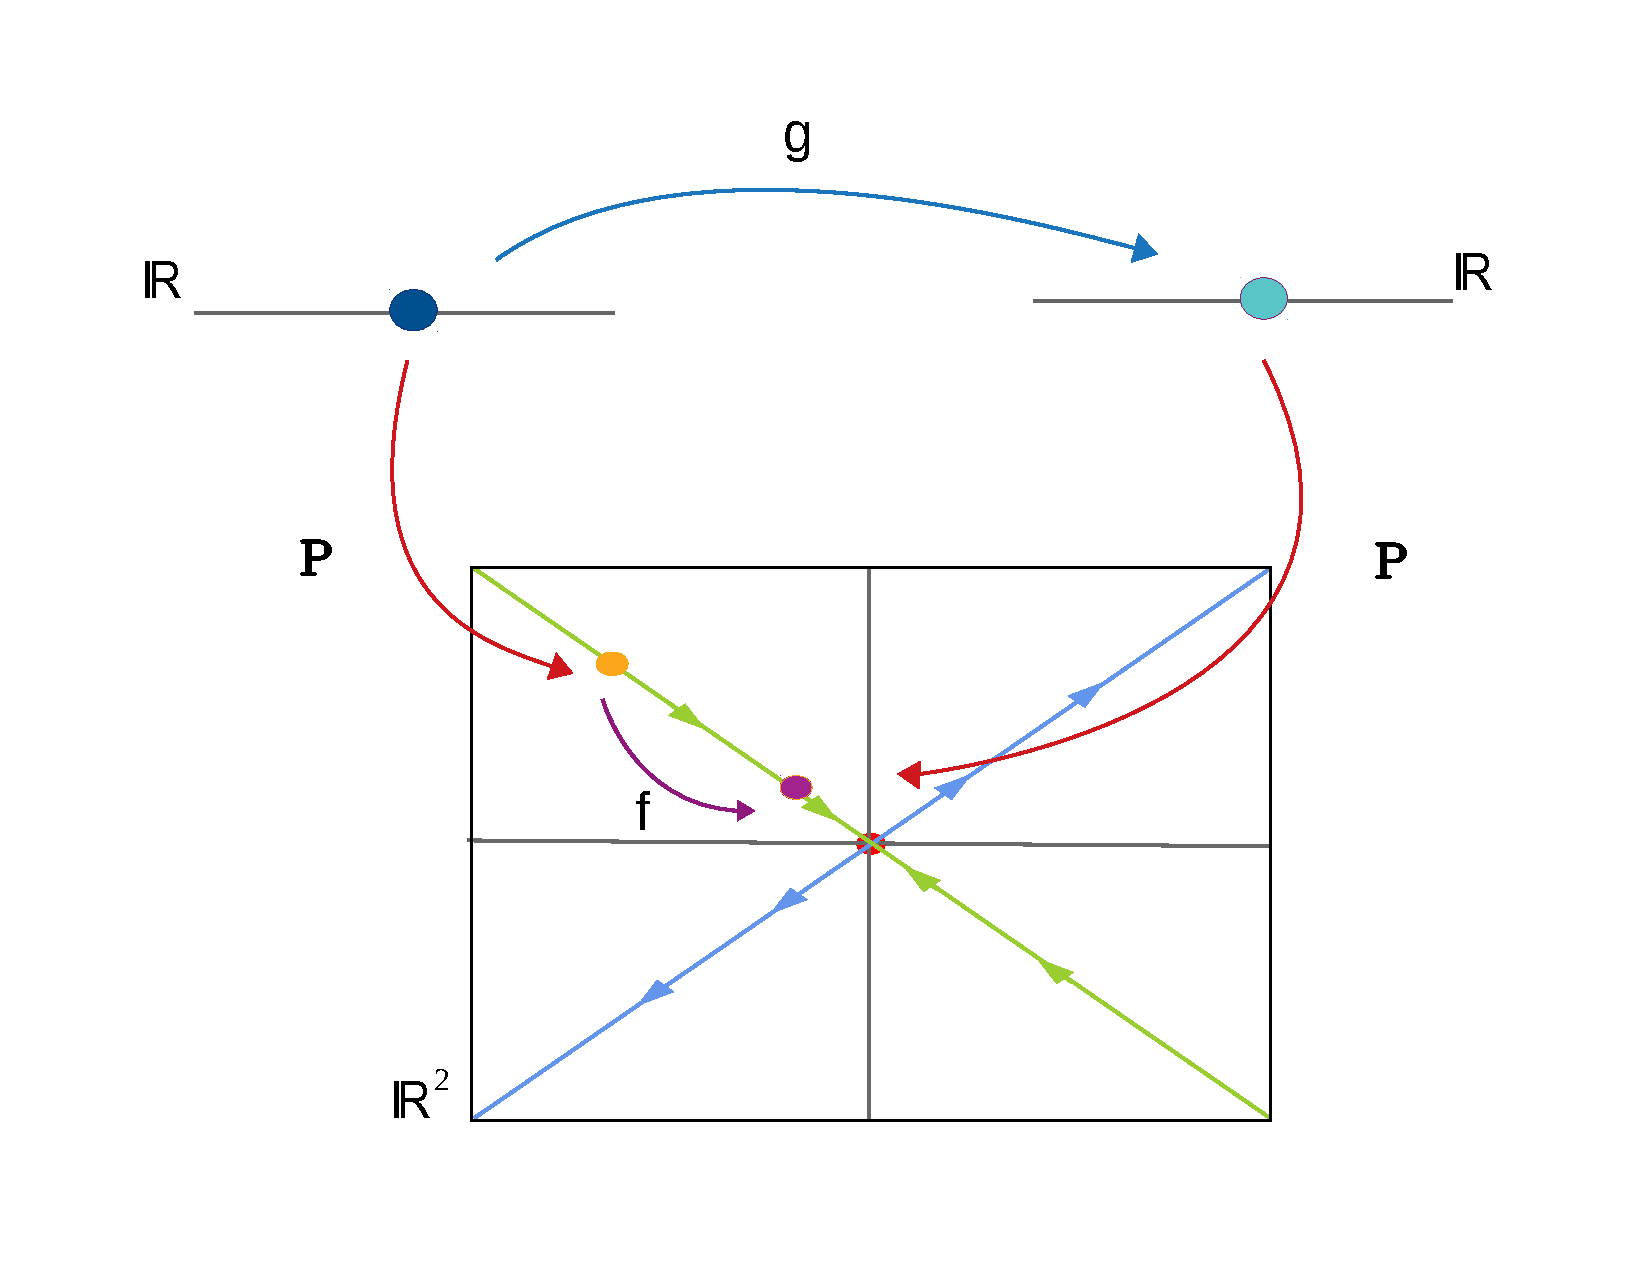
\includegraphics[scale=0.35]{diagrama-c2.pdf}
\end{figure}
\end{frame}

%-----------------------------------------------------------
\begin{frame}
A partir de esto podemos escribir
%\begin{eqnarray}
%\xymatrix{
%\Theta\subset\mathbb{R} \ar[d]^{\mathcal{P}} \ar[r]^{g} & %\Theta\subset\mathbb{R} \ar[d]^{\mathcal{P}} \\
%M\subset\mathbb{R}^{2} \ar[r]^{\mathbf{f}} & %M\subset\mathbb{R}^{2}
%}\label{conmutativo}
%\end{eqnarray}
%de donde obtenemos:
\begin{eqnarray}
\mathbf{f} \circ \mathcal{P} =\mathcal{P}  \circ g
\label{Ecua de invariancia}
\end{eqnarray}
usaremos el m\'etodo gr\'afico.
\begin{equation}
g=\lambda t.
\end{equation}
El error se evalúa como:
\begin{eqnarray}
E_{n}(t) = \parallel \mathbf{f} \circ \mathcal{P}_{n}(t) - \mathcal{P}_{n} \circ g(t) \parallel_{\infty}.  \label{Ecua de invariancia resta}
\end{eqnarray}
\end{frame}



%----------------------------------------------------------

%-------------------------------------------------------------
\begin{frame}{Ejemplo de aplicaci\'on: mapeo est\'andar}
El \textit{mapeo estándar} es
\begin{eqnarray}
\mathbf{f}_{k}(\theta,p) = \left[\begin{array}{c}
\theta + p \\
p + k\sin(\theta +p)
\end{array}\right] \mod(2\pi),  \label{mapeo estandar}
\end{eqnarray}
Puntos fijos:
\begin{itemize}
\item $\mathbf{x}_{1}=(0,0)$
\item $\mathbf{x}_{2}=(0,\pi)$
\end{itemize}
%$\mathbf{f}_{k}(\mathbf{x})=\mathbf{x}$
%con $\mathbf{x}=(\theta,p)$. El resultado de esta condición son unicamente %los puntos $\mathbf{x}_{1}=(0,0)$ y $\mathbf{x}_{2}=(0,\pi)$.

\end{frame}
%--------------------------------------------------------

%\begin{frame}
%Se calcula la derivada total
%\begin{eqnarray}
%D\mathbf{f}_{k}(\theta,p)=\begin{pmatrix}
%1 & 1 \\
%k\cos(\theta+p)& 1+k\cos(\theta+p)\\ 
%\end{pmatrix}.
%\label{mapeo linearizado}
%\end{eqnarray}
%Al evaluar en $\mathbf{x_{1}},\mathbf{x_{2}}$; \eqref{mapeo linearizado} resulta 
%\begin{eqnarray}
%D\mathbf{f}_{k}(0,0)=
%\begin{pmatrix}
%1 & 1\\
%k & 1+k\\
%\end{pmatrix}, \qquad D\mathbf{f}_{k}(0,\pi)= \begin{pmatrix}
%1 & 1\\
%-k & 1-k\\
%\end{pmatrix}.
%\end{eqnarray}


%\end{frame}

%--------------------------------------------------------------
%\begin{frame}
%Se obtienen los valores propios para $\mathbf{x_{1}}$:
%\begin{eqnarray}
%\lambda_{1,2}=\frac{2+k\pm \sqrt{k^{2}+4k}}{2},
%\end{eqnarray}
%cuyos vectores propios $(y_{1},y_{2})$ cumplen que
%\begin{eqnarray}
%y_{2}=y_{1}\left(\frac{1\pm\sqrt{k^{2}+4k}}{2k}\right).
%\label{vectores propios}
%\end{eqnarray}
%En este caso $\mathbf{x}$, es hiperbólico para cualquier $k>0$.\\
%Los valores propios de $\lambda_{2}$ con complejos.
%\end{frame}
%-------------------------------------------------------------
\begin{frame}
Escribimos las variables ($\theta,p$) 
\begin{eqnarray}
\theta(t)=\sum_{n=0}^{\infty}a_{n}t^{n}  ,
\label{theta}
\end{eqnarray}
y
\begin{eqnarray}
p(t)=\sum_{n=0}^{\infty}b_{n}t^{n},
\label{p}
\end{eqnarray}
tal que $\mathcal{P}(t):=(\theta(t),p(t))$.
\end{frame}
%----------------------------------------
\begin{frame}
Sustituyendo en el mapeo est\'andar
\begin{eqnarray}
\mathbf{f}_{k}(\theta,p) = \left[\begin{array}{c}
\theta(t) + p(t) \\
p(t) + k\sin[\theta(t) +p(t)]
\end{array}\right] =\left[ \begin{array}{c}
\theta(\lambda t) \\
p(\lambda t)
\end{array}\right], 
\label{sumas en mapeo}
\end{eqnarray}
de forma expl\'icita es
\begin{eqnarray}
\left[\begin{array}{c}
\sum_{n=0}^{\infty}a_{n}t^{n} + \sum_{n=0}^{\infty}b_{n}t^{n} \\
\sum_{n=0}^{\infty}b_{n}t^{n} + k\sin(\sum_{n=0}^{\infty}a_{n}t^{n} + \sum_{n=0}^{\infty}b_{n}t^{n})
\end{array}\right] =\left[ \begin{array}{c}
\sum_{n=0}^{\infty}a_{n}\lambda^{n}t^{n} \\
\sum_{n=0}^{\infty}b_{n}\lambda^{n}t^{n}
\end{array}\right].
\label{expandida}
\end{eqnarray}
%desarrolando te\'ermino a t\'ermino el primer rengl\'on
%\begin{eqnarray}
%a_{0}+a_{1}t+a_{2}t^{2}+\cdots +b_{0}+b_{1}t+b_{2}t^{2}+ %\cdots=a_{0}+a_{1}\lambda t+\cdots\quad .
%\label{primer renglon}
%\end{eqnarray}

\end{frame}
%----------------------------------------------------
%\begin{frame}
%Usando la serie de Taylor del seno para la segunda ecuaci\'on y %expandiendo las sumas resulta:
%\centering
%\begin{eqnarray*}
%a_{0}+a_{1}t+a_{2}t^{2}+\cdots +b_{0}+b_{1}t+b_{2}t^{2}+ %\cdots=a_{0}+a_{1}\lambda t+\cdots\quad .
%\label{primer renglon}
%\end{eqnarray*}

%\begin{eqnarray*}
%&b_{1}t&+b_{2}t^{2}+\cdots+k\left[a_{0}+(a_{1}+b_{1})t+\cdots\right]-\nonumber\\
%&\frac{k}{3!}&\left[a_{0}+(a_{1}+b_{1})t+(a_{2}+b_{2})t^{2}+\cdots\right]^{3}+\cdots\nonumber\\
%&=&b_{1}\lambda t+b_{2}\lambda^{2}t^{2}+\cdots
%\label{segundo renglon}
%\end{eqnarray*}
%\end{frame}
%\begin{eqnarray}
%\sum_{n=0}^{\infty}b_{n}t^{n} %+k\sum_{j=0}^{\infty}\frac{(-1)^{j}}{(2j+1)!}\left[ %\sum_{n=0}^{\infty}a_{n}t^{n} %+\sum_{n=0}^{\infty}b_{n}t^{n}\right]^{2j+1}=\sum_{n=0}^{\infty}b_{n}\lambda^{n%}t^{n}.
%\label{seno exapandido 2}
%\end{eqnarray}
%Desarrollando las sumas
%\begin{eqnarray}
%&b_{1}t&+b_{2}t^{2}+\cdots+k\left[a_{0}+(a_{1}+b_{1})t+\cdots\right]-\nonumber\\
%&\frac{k}{3!}&\left[a_{0}+(a_{1}+b_{1})t+(a_{2}+b_{2})t^{2}+\cdots\right]^{3}+\cdots\nonumber\\
%&=&b_{1}\lambda t+b_{2}\lambda^{2}t^{2}+\cdots
%\label{segundo renglon}
%\end{eqnarray}
%\end{frame}
%------------------------------------------------------------

%-----------------------------------------------------
\begin{frame}
Comparamos t\'erminos del mismo orden
\begin{itemize}
\item Orden cero:
\begin{equation}
a_{0}+b_{0}=a_{0} \rightarrow b_{0}=0
\end{equation}
\begin{equation}
k a_{0}+\frac{k}{3!}a_{0}^{3}+\cdots=0  \rightarrow a_{0}=0
\end{equation}
\item  Orden uno:
\begin{eqnarray}
a_{1}+b_{1}=a_{1}\lambda ,
\end{eqnarray}

\begin{eqnarray}
b_{1}+ka_{1}+b_{1}=b_{1}\lambda .
\end{eqnarray}
\item Orden dos:
\begin{eqnarray}
a_{2}+b_{2}=a_{2}\lambda^{2}.
\label{segundos_coeficientes_a}
\end{eqnarray}
\begin{eqnarray}
b_{2}+ka_{2}+b_{2}=b_{2}\lambda^{2}.
\label{segundos_coeficientes_b}
\end{eqnarray}
\end{itemize}

\end{frame}


%---------------------------------------------------------
%\begin{frame}
%Ocuparemos un truco, buscaremos que la ecuaci\'on \eqref{expandida} %satisfaga una ecuaci\'on diferencial simple. Para ello escribimos a $W$ %como:
%\begin{eqnarray}
%W(t)=\sum_{n=0}^{\infty}\beta_{n}t^{n}=\sin\left(\sum_{n=0}^{\infty}a_{n}t^%{n}+\sum_{n=0}^{\infty}
%b_{n}t^{n}\right).
%\end{eqnarray}
%Consideramos como un compleja a $W$
%\begin{eqnarray}
%\overline{W}=\sum_{n=0}^{\infty}(\alpha_{n}+i\beta_{n})t^{n}=\exp[i(\theta(%t)+p(t))],
%\label{W compleja}
%\end{eqnarray}
%Ya que $W(t)=Im(\overline{W})$.\\
%Al tomar la derivada de \eqref{W compleja}
%\begin{eqnarray}
%\overline{W}'=i\overline{W}[\theta '(t)+p'(t)].
%\label{W compleja deriv}
%\end{eqnarray}
%\end{frame}
%------------------------------------------------------------------------
%\begin{frame}
%Hay otra forma de calcular los coeficientes: mediante relaciones de recurrencia. Para ello se usa el truco de buscar que la ecuación \eqref{expandida} satisfaga una ecuación diferenical simple. Para ello proponemos:
%\begin{eqnarray}
%W(t)=\sum_{n=0}^{\infty}\beta_{n}t^{n}=\sin\left(\sum_{n=0}^{\infty}a_{n}t^{n}+\sum_{n=0}^{\infty}
%b_{n}t^{n}\right).
%\end{eqnarray}
%Consideramos como un compleja a $W$
%\begin{eqnarray}
%\overline{W}=\sum_{n=0}^{\infty}(\alpha_{n}+i\beta_{n})t^{n}=\exp[i(\theta(t)+p(t))],
%\label{W compleja}
%\end{eqnarray}
%Ya que $W(t)=Im(\overline{W})$.\\
%Al tomar la derivada de \eqref{W compleja}
%\begin{eqnarray}
%\overline{W}'=i\overline{W}[\theta '(t)+p'(t)].
%\label{W compleja deriv}
%\end{eqnarray}
%\end{frame}
%---------------------------------------------------------
\begin{frame}

Hay otra forma de calcular los coeficientes: mediante relaciones de recurrencia. Para ello se usa el truco de buscar que la ecuación \eqref{expandida} satisfaga una ecuaci\'on diferencial simple.
\begin{eqnarray}
\alpha_{n+1}=\frac{-1}{n+1}\sum_{l=0}^{n}(l+1)\beta_{n-l}(a_{l+1}+b_{l+1}),
\label{recurrencia alpha}
\end{eqnarray}
\begin{eqnarray}
\beta_{n+1}=\frac{1}{n+1}\sum_{l=0}^{n}(l+1)\alpha_{n-l}(a_{l+1}+b_{l+1}),
\label{recurrencia beta}
\end{eqnarray}
\begin{eqnarray}
a_{n+1}=\frac{k}{(n+1)[(1-\lambda^{n+1})(1-\lambda^{n+1}+k)-k]}\sum_{l=0}^{n-1}\alpha_{n-l}(l+1)(a_{l+1}+b_{l+1}),
\end{eqnarray}
\begin{eqnarray}
b_{n+1}=\frac{-k 1-\lambda^{n+1}}{(n+1)[(1-\lambda^{n+1})(1-\lambda^{n+1}+k)-k]}\sum_{l=0}^{n-1}\alpha_{n-l}(l+1)(a_{l+1}+b_{l+1}).
\end{eqnarray}
\end{frame}
%----------------------------------------------------------
%\begin{frame}

%\end{frame}
%-------------------------------------------------------
%\begin{frame}
%Mucha talacha!\\
%Expandiendo en potencias de $t$ la ecuaci\'on \eqref{W compleja deriv}, se %obtiene
%\begin{eqnarray}
%\sum_{n=0}^{\infty}(n+1)(\alpha_{n+1}+i\beta_{n+1})t^{n}=i\sum_{n=0}^{\inft%y}c_{n}t^{n}+i\sum_{n=0}^{\infty}d_{n}t^{n},
%\end{eqnarray}
%con
%\begin{eqnarray}
%c_{n}=\sum_{l=0}^{n}(l+1)(\alpha_{n-l}+i\beta_{n-l})a_{l+1}, \\
%d_{n}=\sum_{l=0}^{n}(l+1)(\alpha_{n-l}+i\beta_{n-l})b_{l+1}.
%\end{eqnarray}

%\end{frame}
%---------------------------------------------------
%\begin{frame}
%Separando la parte real 
%\begin{eqnarray}
%\sum_{n=0}^{\infty}(n+1)\alpha_{n+1}t^{n}=\sum_{n=0}^{\infty}\left[-\sum_{l%=0}^{n}(l+1)\beta_{n-l}(a_{l+1}+b_{l+1})\right]t^{n},
%\label{parte real}
%\end{eqnarray}
%e imaginaria
%\begin{eqnarray}
%\sum_{n=0}^{\infty}(n+1)\beta_{n+1}t^{n}=\sum_{n=0}^{\infty}\left[\sum_{l=0%}^{n}(l+1)\alpha_{n-l}(a_{l+1}+b_{l+1})\right]t^{n}.
%\label{parte compleja}
%\end{eqnarray}
%\end{frame}

%-----------------------------------------------------------
%\begin{frame}
%Igualando potencias de $t$ en \eqref{parte real}, \eqref{parte compleja} y despejando $\alpha_{n+1},\beta_{n+1}$ se obtiene
%Igualando potencias de $t$ en \eqref{W compleja deriv} y %despejando $\alpha_{n+1},\beta_{n+1}$ se obtiene
%\begin{eqnarray}
%\alpha_{n+1}=\frac{-1}{n+1}\sum_{l=0}^{n}(l+1)\beta_{n-l}(%a_{l+1}+b_{l+1}),
%\label{recurrencia alpha}
%\end{eqnarray}
%\begin{eqnarray}
%\beta_{n+1}=\frac{1}{n+1}\sum_{l=0}^{n}(l+1)\alpha_{n-l}(a_{l+1}+b_{l+1}),
%\label{recurrencia beta}
%\end{eqnarray}

%Usando el caso $t=0$ en la ecuación \eqref{W compleja} %resulta
%\begin{eqnarray}
%\overline{W}(0)=\alpha_{0}+i\beta_{0}=\cos(\theta(0)+p(0))+i\sin(\theta(0)+p(0))=1,
%\end{eqnarray}
%por lo que $\alpha_{0}=1,\beta_{0}=0$.
%\end{frame}

%----------------------------------------------------
%\begin{frame}
%Para encontrar los otros coeficientes usamos de nuevo la ecuaci\'on del %mapeo, considerando lo que propusimos para el t\'ermino del seno
%\begin{eqnarray}
%\sum_{n=1}^{\infty}a_{n}t^{n}+\sum_{n=1}^{\infty}b_{n}t^{n}=\sum_{n=1}^{\in%fty}a_{n}\lambda^{n}t^{n},
%\end{eqnarray}
%\begin{eqnarray}
%\sum_{n=1}^{\infty}b_{n}t^{n}+k\sum_{n=1}^{\infty}\beta_{n}t^{n}=\sum_{n=1}%^{\infty}b_{n}
%\lambda^{n}t^{n}.
%\end{eqnarray}
%\end{frame}
%---------------------------------------------------
%\begin{frame}
%Al agrupar los t\'erminos de orden $n+1$ en ambas ecuaciones resulta:
%\begin{eqnarray}
%\mathbf{A}\begin{pmatrix}
%a_{n+1}\\
%b_{n+1}
%\end{pmatrix}=-\frac{k}{n+1}\sum_{l=0}^{n-1}(l+1)\alpha_{n-l}(a_{l+1}+b_{l+1})\begin{pmatrix}
%0\\
%1
%\end{pmatrix},
%\label{sistema recurrencia}
%\end{eqnarray}
%siendo 
%\begin{eqnarray}
%\mathbf{A}=\begin{pmatrix}
%a-\lambda^{n+1} & 1 \\
%k & 1-\lambda^{n+1}+k
%\end{pmatrix}.
%\end{eqnarray}
%\end{frame}
%---------------------------------------------------------
%\begin{frame}
%Sustituyendo $\sum_{n=0}^{\infty}\beta_{n}t^{n}$ en lugar del seno, agrupamos términos de orden $n+1$ y despejamos $a_{n+1},b_{n+1}$, para obtener:
%\begin{eqnarray}
%a_{n+1}=\frac{k}{(n+1)[(1-\lambda^{n+1})(1-\lambda^{n+1}+k)-k]}\sum_{l=0}^{n-1}\alpha_{n-l}(l+1)(a_{l+1}+b_{l+1}),
%\end{eqnarray}
%\begin{eqnarray}
%b_{n+1}=\frac{-k 1-\lambda^{n+1}}{(n+1)[(1-\lambda^{n+1})(1-\lambda^{n+1}+k)-k]}\sum_{l=0}^{n-1}\alpha_{n-l}(l+1)(a_{l+1}+b_{l+1}).
%\end{eqnarray}
%\end{frame}

%-----------------------------------------------------
\begin{frame}{Iterativo}
\begin{figure}
	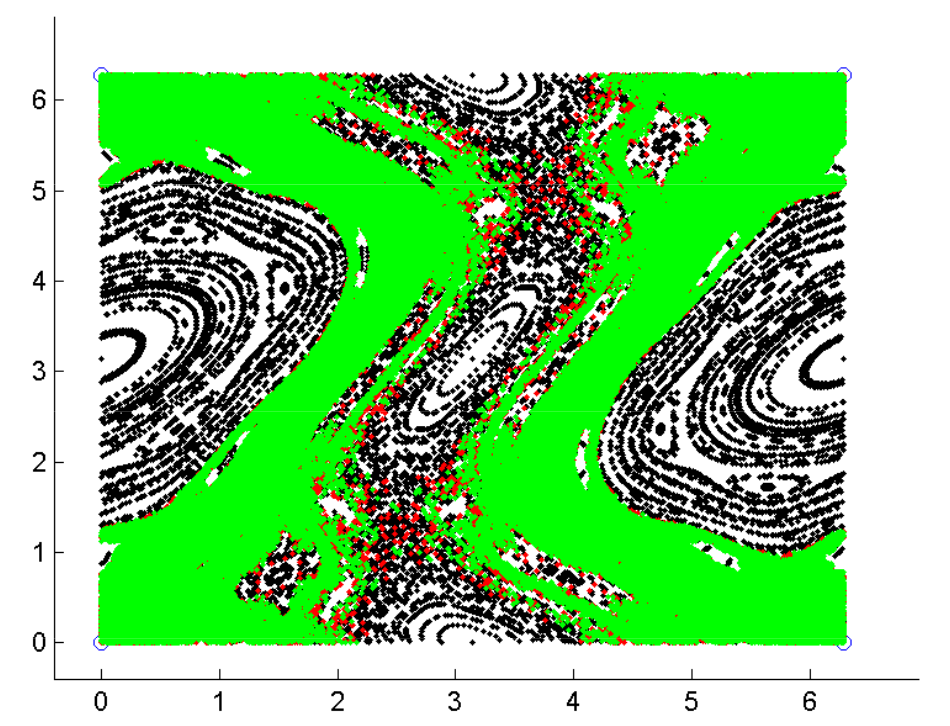
\includegraphics[scale=0.25]{iteradosMireles.png}
	\caption{Variedades calculadas mediante iterar un conjunto de condiciones iniciales 300 veces. \cite{Mireles}}
\end{figure}

\end{frame}
%_________________________________________________________
\begin{frame}{Ejemplos de aplicaci\'on: mapeo est\'andar}
Usando el punto fijo  $\mathbf{x}_{1}=(0,0)$.
\begin{figure}[H]
\centering
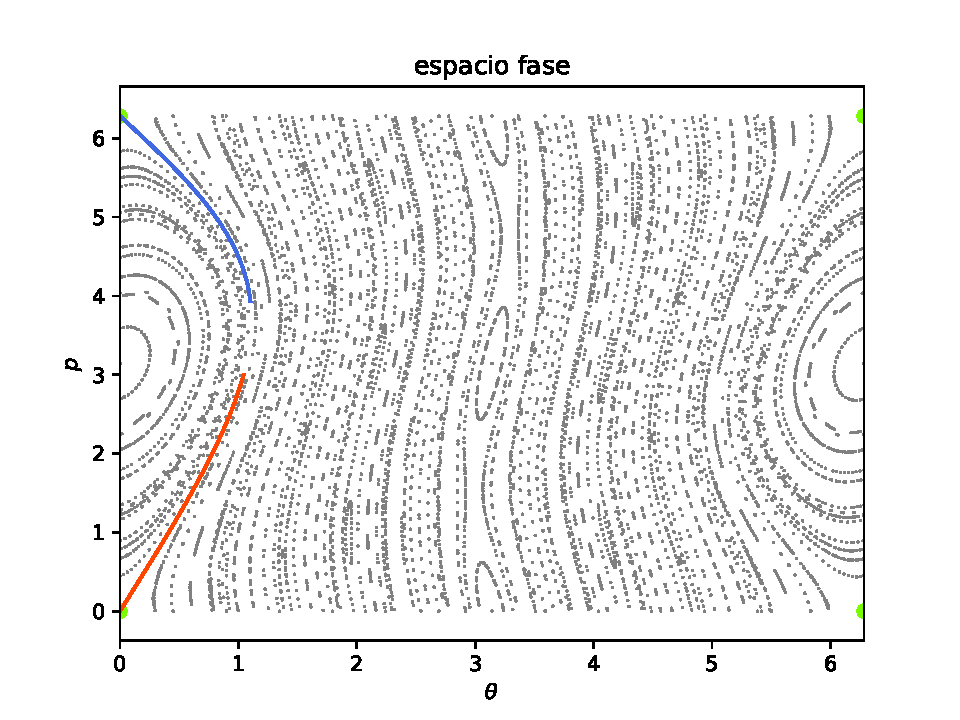
\includegraphics[scale=0.4]{k03}
\caption{\footnotesize $W^{s},W^{u}$ de orden $25$ en el mapeo estándar con $k=0.3$ en el intervalo $t=[0.,3.]$}
\label{estandar03}
\end{figure}
\end{frame}
%---------------------------------------------------------------------
\begin{frame}
El error:
%\begin{eqnarray*}
%E_{n}(t) = \parallel \mathbf{f} \circ \mathcal{P}_{n}(t) - %\mathcal{P}_{n} \circ g(t) \parallel_{\infty}.
%\label{Ecua de invariancia resta}
%\end{eqnarray*}
\begin{figure}[H]
\centering
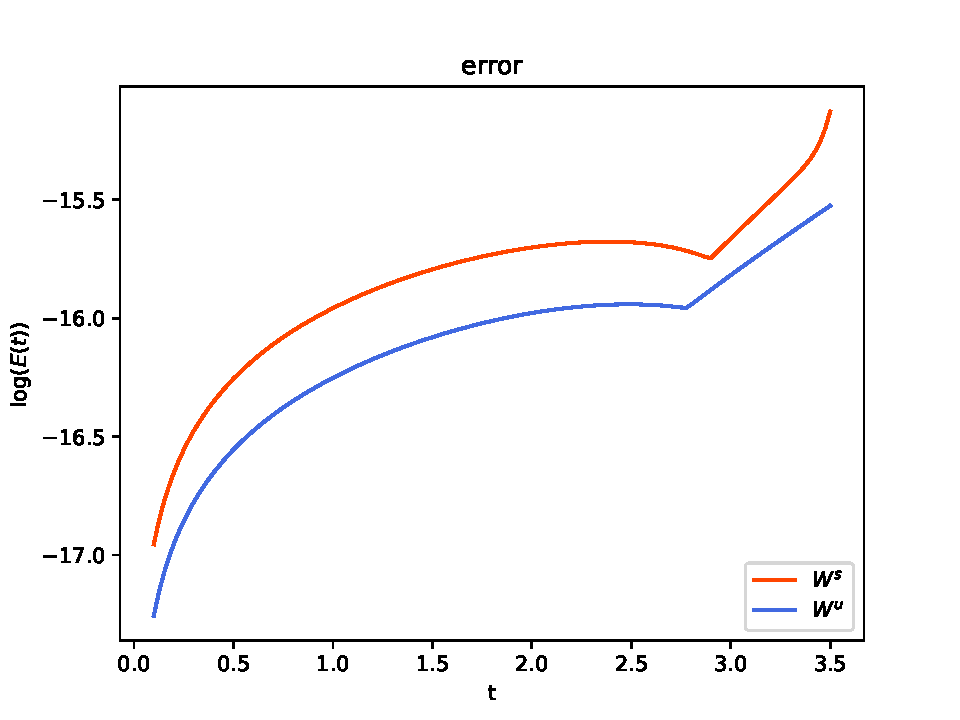
\includegraphics[scale=0.5]{errork03} 
\caption{Error en las variedades de la figura \ref{estandar03}.}
\label{error est k03}
\end{figure}
\end{frame}
%---------------------------------------------------------
\begin{frame}
\begin{figure}[H]
\centering
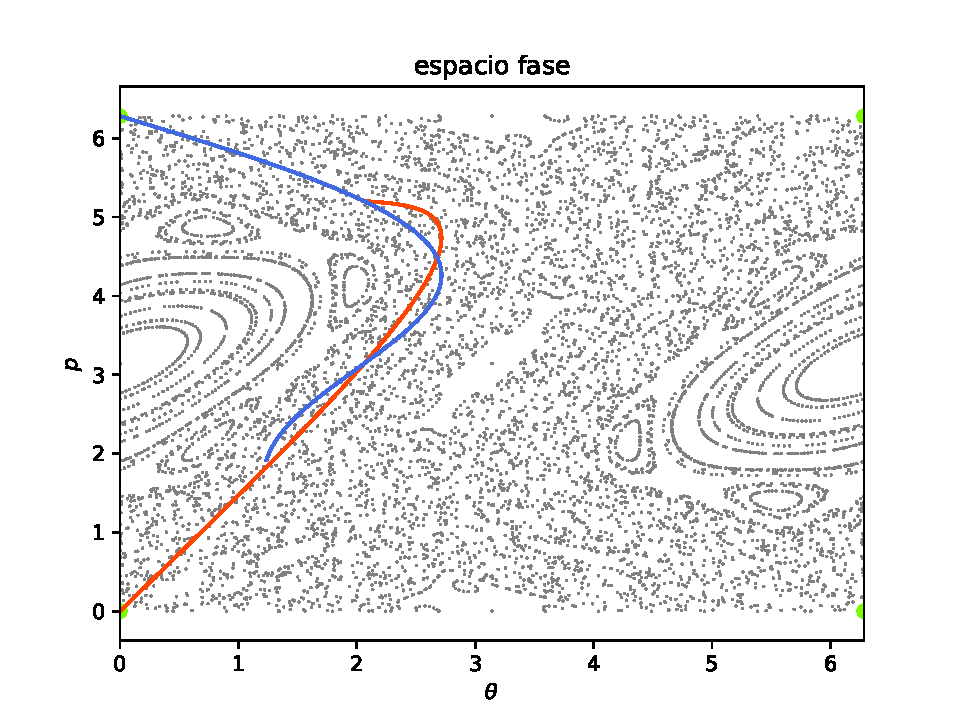
\includegraphics[scale=0.35]{k15}
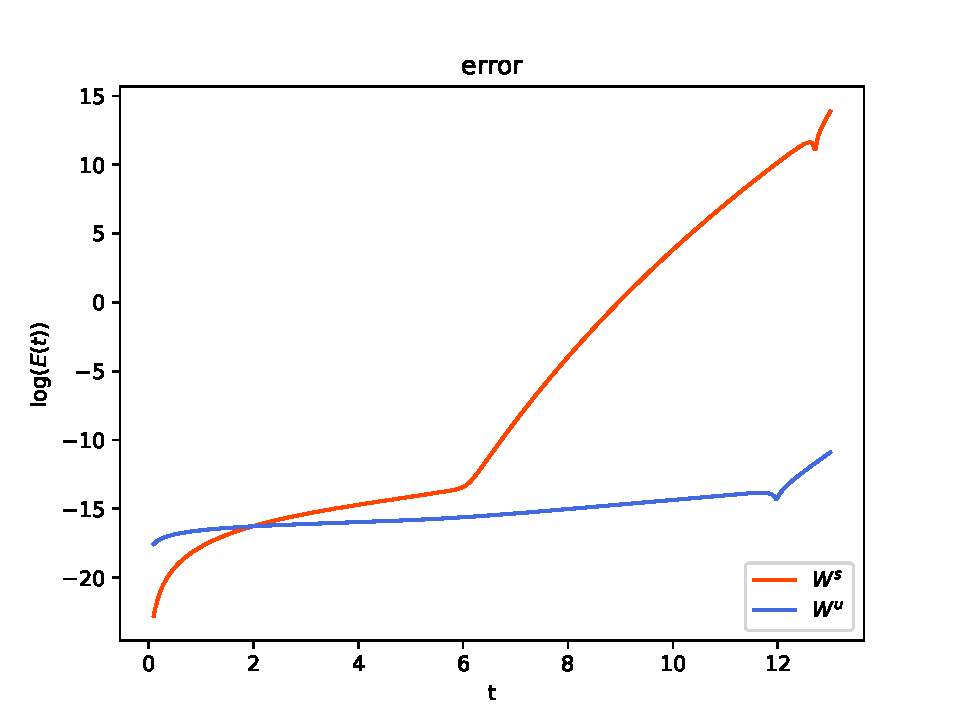
\includegraphics[scale=0.35]{errork15}
\caption{$W^{s},W^{u}$ de orden $80$ en el mapeo estándar con $k=1.5$ en el intervalo $t=[0.,13.]$ y su error.}
\label{estandar15}
\end{figure}
\end{frame}


%--------------------------------------------------------------
\begin{frame}
Para observar c\'omo cambia el error con el orden de la parametrizaci\'on.
\begin{figure}[H]
\centering
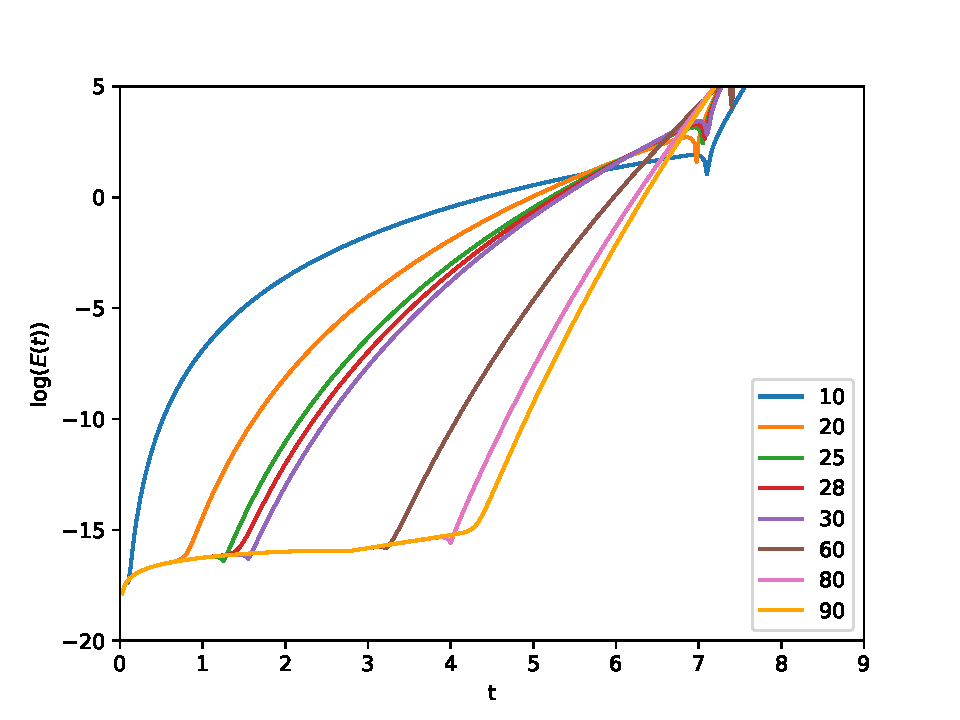
\includegraphics[scale=0.5]{errorf64}
\caption{Curvas de error para diferentes órdenes en el mapeo estándar, $k=0.3$. }
\label{erroresf64}
\end{figure}
\end{frame}

%--------------------------------------------------------------------
\begin{frame}
Usando n\'umeros de presici\'on extendida
\begin{figure}[H]
\centering
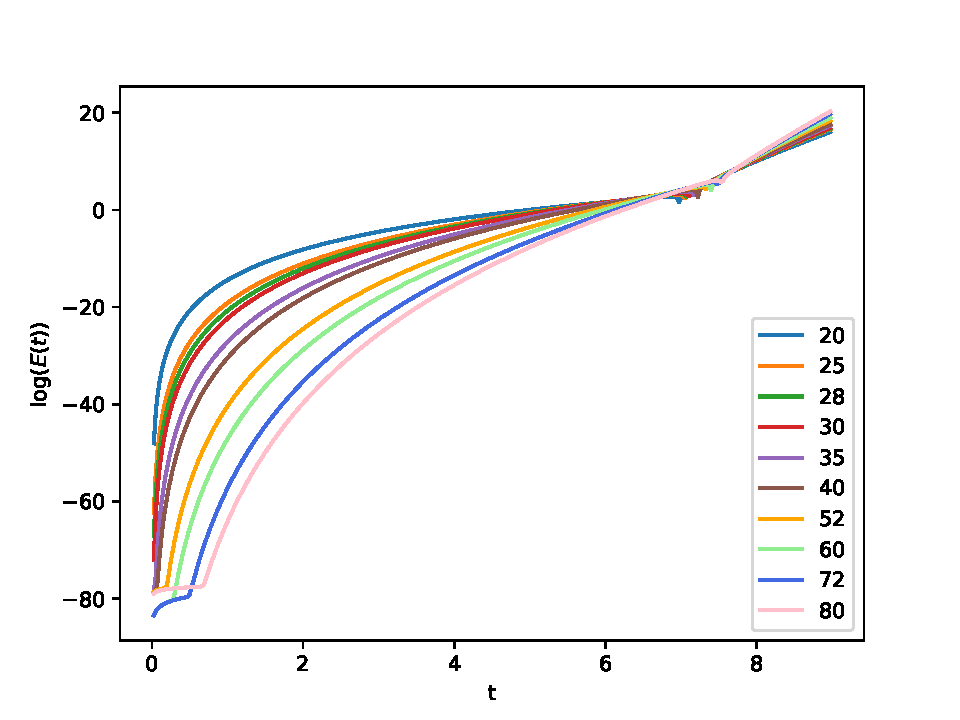
\includegraphics[scale=0.6]{errorbf}
\caption{Curvas de error para diferentes órdenes usando precisión extendida ,$k=0.3$. }
\label{erroresBig}
\end{figure}
\end{frame}

%-------------------------------------------------------------------
\begin{frame}
Usando mapeo est\'andar inverso
\begin{eqnarray}
\mathbf{f}_{k}^{-1}(p,\theta) = \left[\begin{array}{c}
p  -k\sin(\theta) \\
\theta-p+k\sin{\theta}
\end{array}\right] \mod(2\pi), \label{mapeo estandar inverso}
\end{eqnarray}
podemos calcular la varieda estable
\begin{figure}[H]
\centering
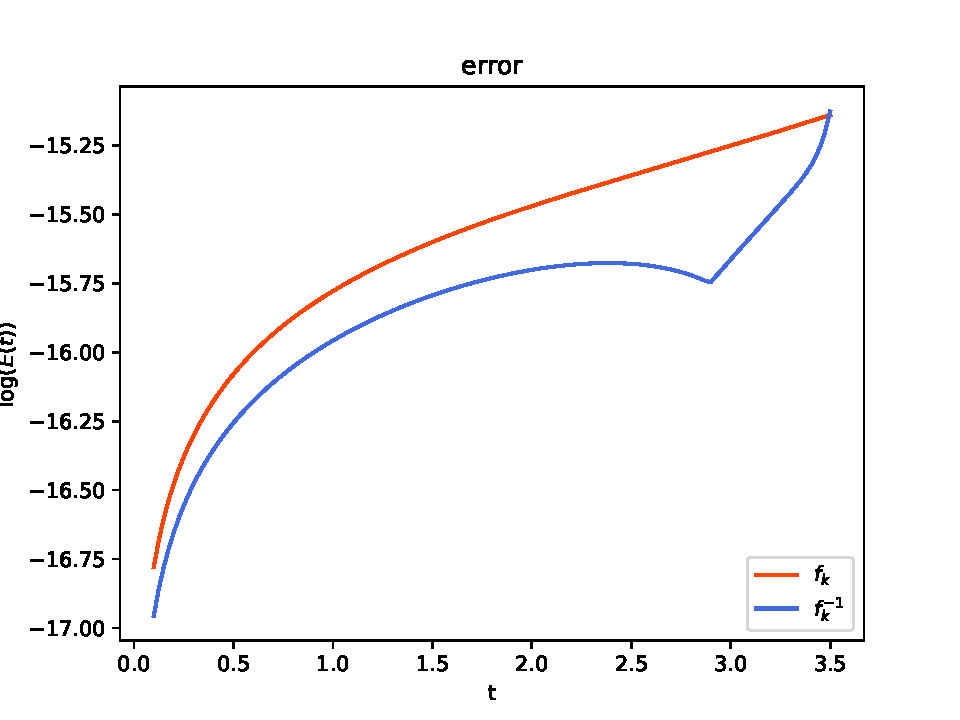
\includegraphics[scale=0.4]{error_inversa}
\caption{Error para las parametrizaciones usando el mapeo y el mapeo inverso con polinomios de orden $20$ y $k=0.3$. }
\label{erroresinverso}
\end{figure}
\end{frame}
%-------------------------------------------------------------
\begin{frame}{Mapeo de H\'enon}
El mapeo de Hénon se define como:
\begin{eqnarray}
\mathbf{f}_{a,b}(x,y)=\left( \begin{array}{lcc}
a-by-x^{2}\\
\\ x
\end{array}
\right), \label{Henon}
\end{eqnarray}

y su inverso:
\begin{eqnarray}
\mathbf{f}^{-1}_{a,b}(x,y)=\left( \begin{array}{lcc}
y\\
\\ (a-x-y^{2})/b
\end{array}
\right). \label{HenonI}
\end{eqnarray} 


\end{frame}

%--------------------------------------------------------------
\begin{frame}
\begin{figure}[H]
\centering
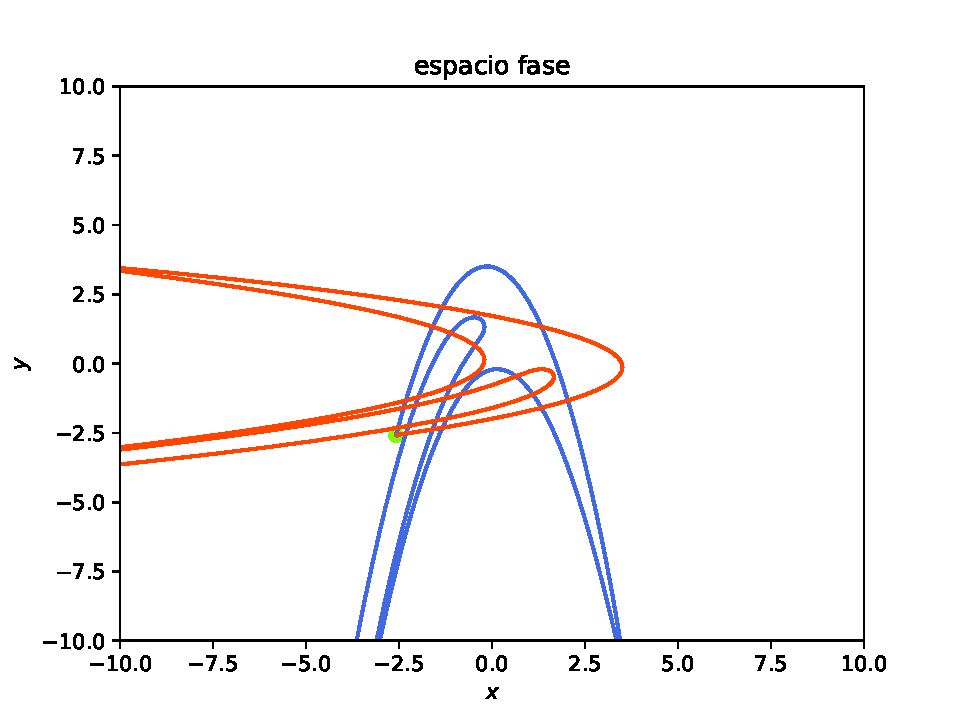
\includegraphics[scale=0.35]{h15}
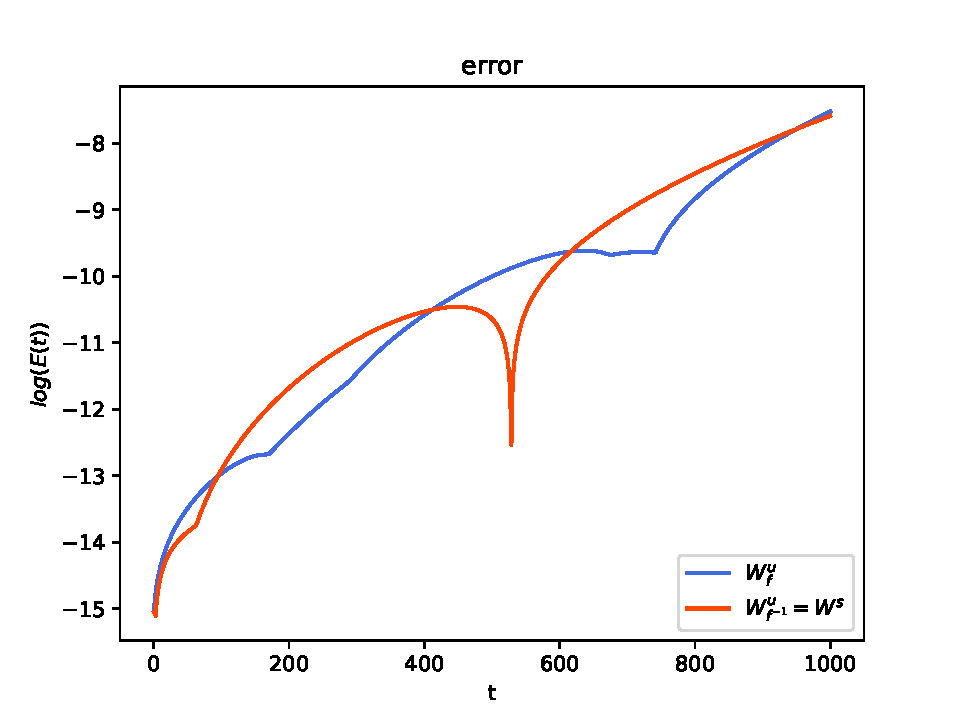
\includegraphics[scale=0.35]{errorH15}
\caption{$W^{u}$ y $W^{s}$ de orden 45 en el intervalo $t=[0.,900.]$ para el mapeo de Hénon con $a=1.5$,$b=1$.}
\label{Henon1}
\end{figure}

\end{frame}

%-------------------------------------------------------------------
\begin{frame}
\begin{figure}
\centering
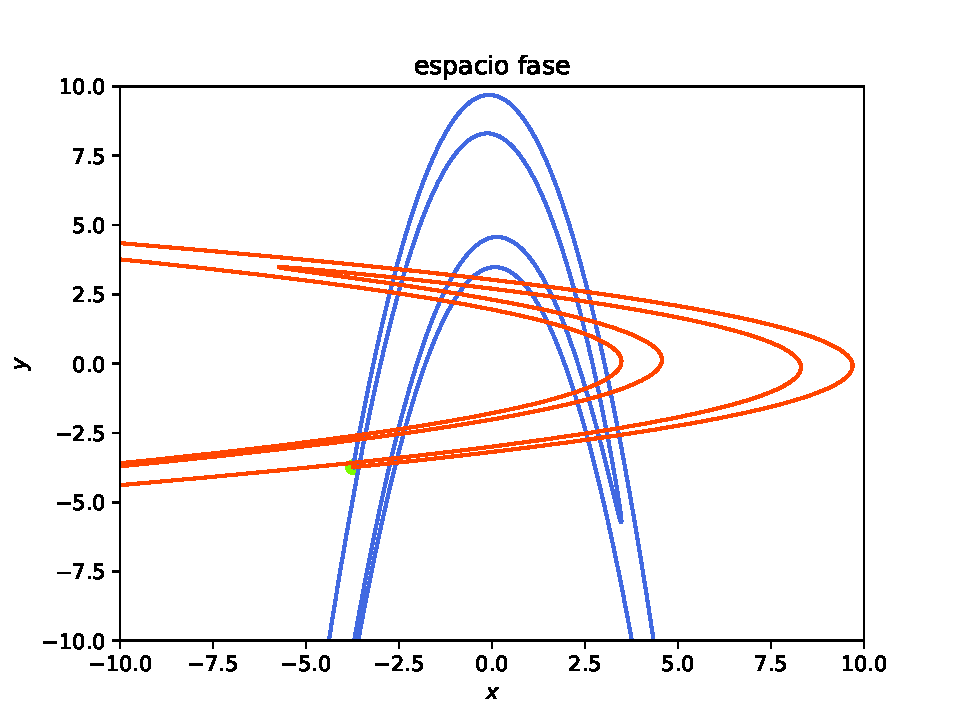
\includegraphics[scale=0.35]{h65}
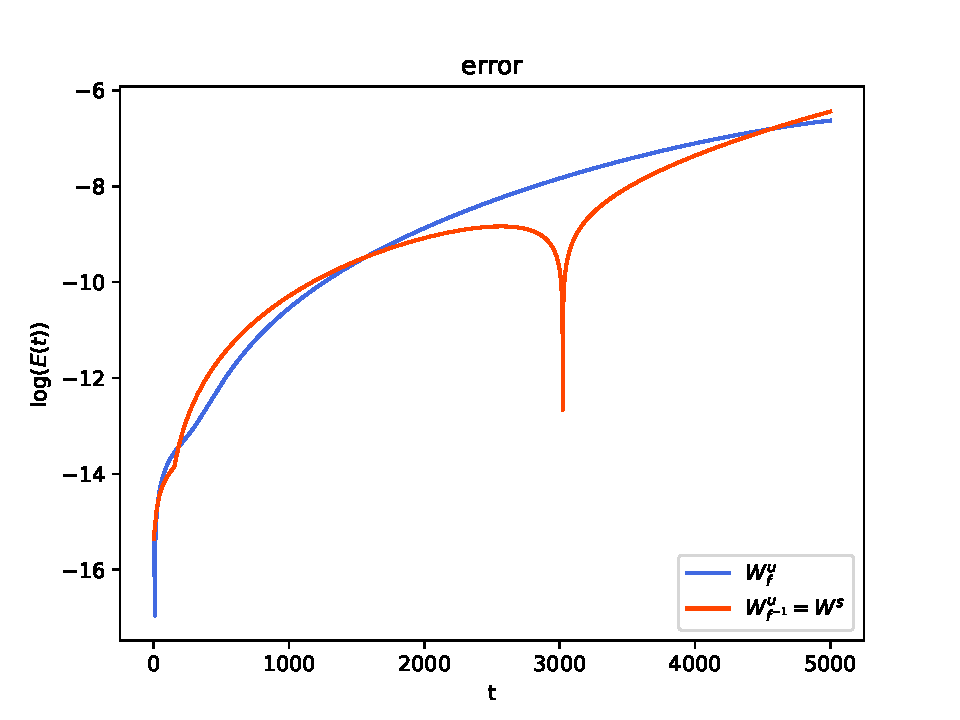
\includegraphics[scale=0.35]{errorH65}
\caption{$W^{u}$, $W^{s}$ de orden $78$ en el intervalo $t=[0.,4000.0]$ para el mapeo de Hénon con $a=6.5$,$b=1.$.}
\label{Henon3}
\end{figure}

\end{frame}
%------------------------------------------

\begin{frame}{Mapeo exponencial}
El mapeo exponencial se define como:
\begin{eqnarray}
\mathbf{j}_{a}(x,y)=\left(\begin{array}{lcc}
x+y\\
\\ y+af(x+y)
\end{array}\right), \quad f(x)=x(x-1)e^{-x}.
\label{Jung}
\end{eqnarray}
y su inverso
\begin{eqnarray}
\mathbf{j}^{-1}_{a}(x,y)=\left(\begin{array}{lcc}
x-y+ax(x-1)e^{-x}\\
\\ y-ax(x-1)e^{-x}
\end{array}\right)
\label{jungI}
\end{eqnarray}
Los puntos fijos del sistema son:
\begin{itemize}
\item $\mathbf{x}_{0}=(1,0) \rightarrow$ hiperb\'olico
\item $\mathbf{x}_{1}=(0,0)$  
\begin{itemize}
\item el\'iptico si $a<4$
\item inverso hiperb\'olico si $a \geq 4$
\end{itemize}
\end{itemize}

\end{frame}

\begin{frame}
\begin{figure}[H]
\centering
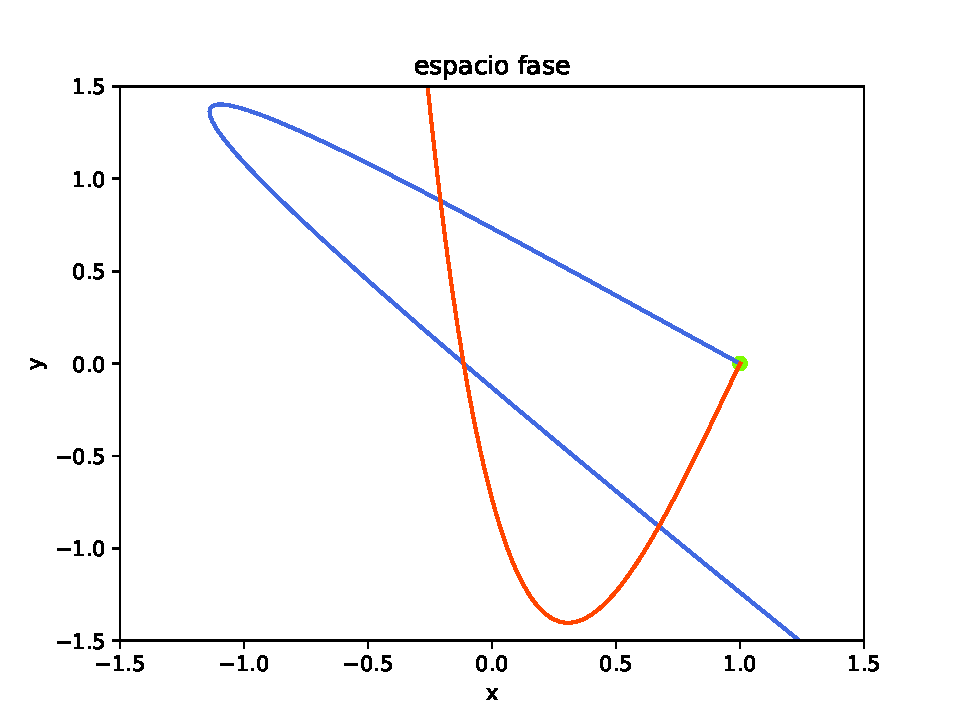
\includegraphics[scale=0.35]{jung57}
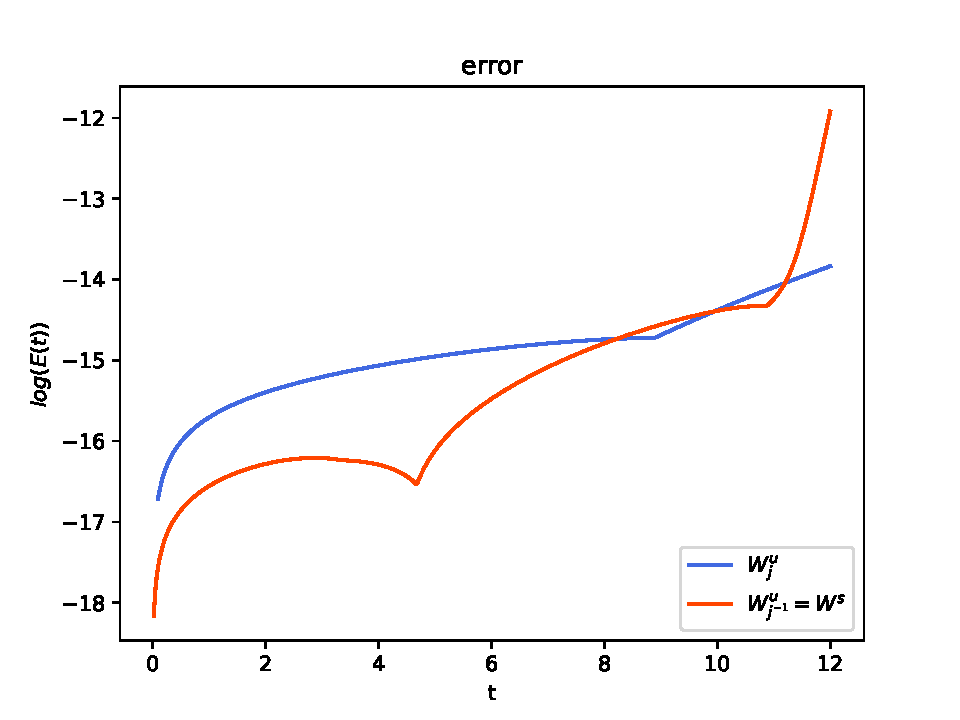
\includegraphics[scale=0.35]{error_jung57}
\caption{$W^{s}$ y $W^{u}$ de orden 93 en el intervalo $t=[0.,6.5]$, con $a=5.7$ en el punto fijo $x_{0}$.}
\label{jung2}
\end{figure}

\end{frame}
%--------------------------------------------------------------
%-------------------------------------------------------------
\begin{frame}{Convergencia}
Usando el criterio de Hadamard
\begin{eqnarray}
\lim_{n\rightarrow\infty}\frac{a_{n}}{a_{n+1}},\label{hadamard}
\end{eqnarray} 
\begin{figure}
\centering
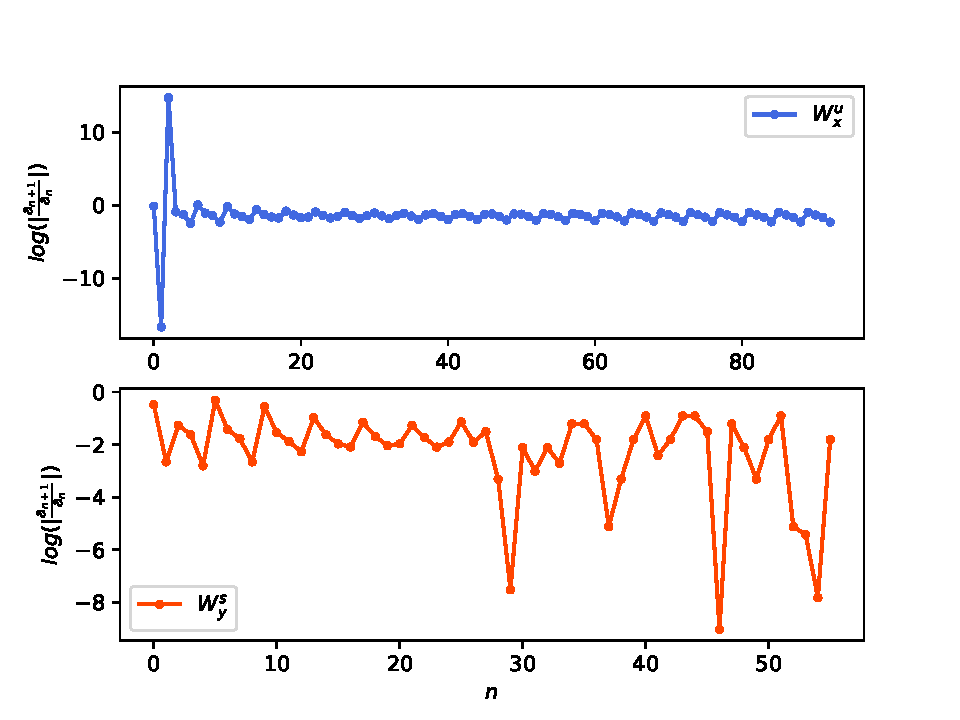
\includegraphics[scale=0.4]{convergenciaJungH57}
\caption{Convergencia de Hadamard asociada a las variedades mostradas en la figura \ref{jung2}.}
\label{convergenciaJH}
\end{figure}


\end{frame}
%------------------------------------------------------------------
\begin{frame}
Usando el criterio de los tres t\'erminos:
\begin{eqnarray}
\lim_{i\rightarrow\infty} \left[ i\left(\frac{a_{i+1}}{a_{i}}\right)-(i-1)\left(\frac{a_{i}}{a_{i-1}}\right) \right].
\label{tres terminos}
\end{eqnarray}
\begin{figure}
\centering
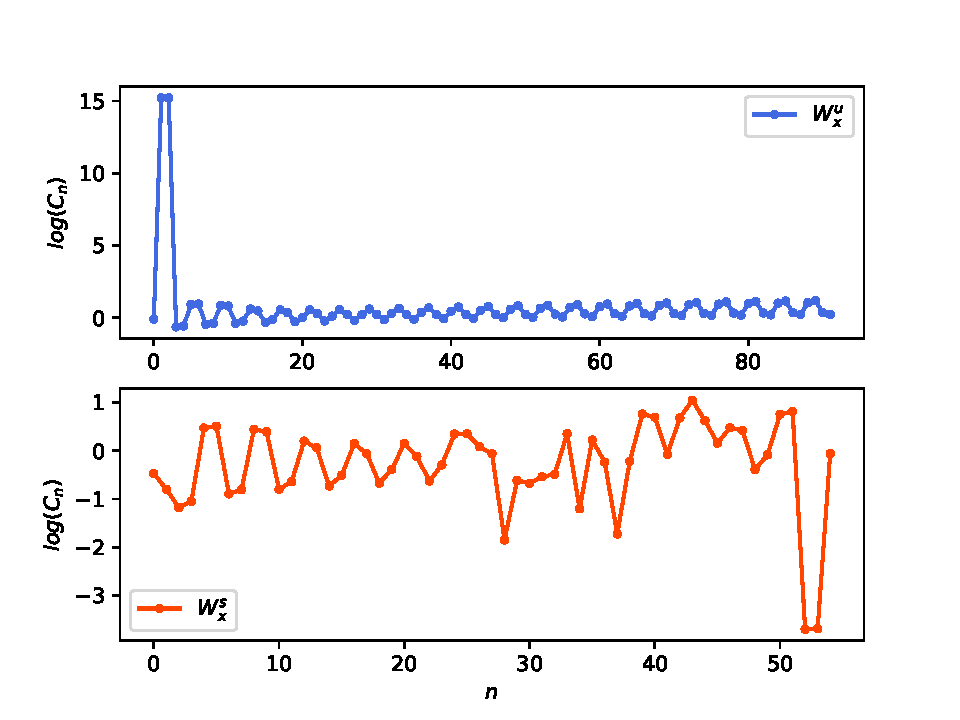
\includegraphics[scale=0.4]{convergenciaJungT57}
\caption{Convergencia de tres términos asociada a las variedades en la figura \ref{jung2}.}
\label{convergenciaJ3}
\end{figure}
\end{frame}
%------------------------------------------------------------------------
\begin{frame}{Existencia de puntos homocl\'inicos}
\justifying
Siendo que el resultado son polinomios, se puede aplicar el método de Newton, o cualquier otro, en dos dimensiones para resolver $\mathcal{P}^{u}=\mathcal{P}^{s}$.
Concretamente se tienen \\
\begin{equation}
W^{s}(t)=(\mathcal{P}_{x}(t),\mathcal{P}_{y}(t)) ,\quad W^{u}(\tau)=(\mathcal{P}_{x}(\tau),\mathcal{P}_{y}(\tau))
\end{equation}
\begin{eqnarray}
W^{s}(t)=W^{u}(\tau),
\end{eqnarray}
\justifying
la intersección se encontrará en $I_{t}\times I_{\tau}$. En el espacio fase la intersección se verá como el producto cartesiano de $W^{s}(I_{t})\times W^{u}(I_{\tau})$ formando una sección en la que se garantiza hay un punto homoclínico o heteroclínico. 
\end{frame}
%----------------------------------------------------------------------
\begin{frame}{Est\'andar}
\begin{figure}
\centering
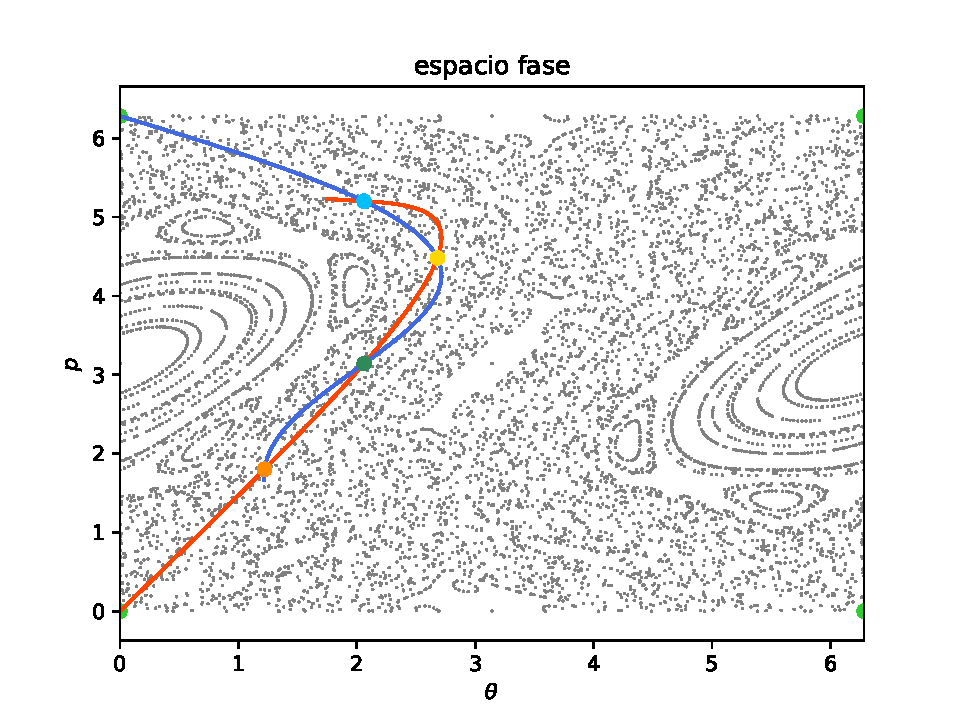
\includegraphics[scale=0.5]{cruce_estandar}
\caption{Cruces de $W^{u},W^{s}$ de orden $120$ para el mapeo estándar con $k=1.5$, usando una tolerancia de $10^{-6}$.}
\label{cruce_estandar}
\end{figure}

\end{frame}
%---------------------------------------------------------------------------
\begin{frame}{H\'enon}
\begin{figure}
\centering
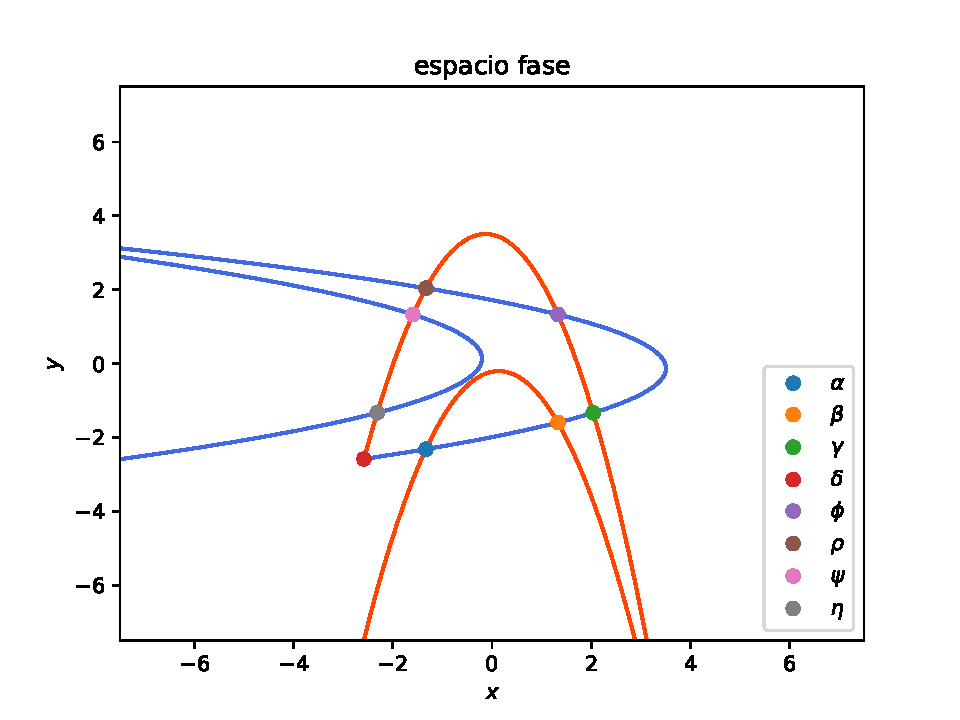
\includegraphics[scale=0.5]{crucesL}
\caption{Cruces de $W^{u},W^{s}$ , con una tolerancia de $10^{-6}$.}
\label{crucesH}
\end{figure}
\end{frame}

\begin{frame}
\begin{figure}
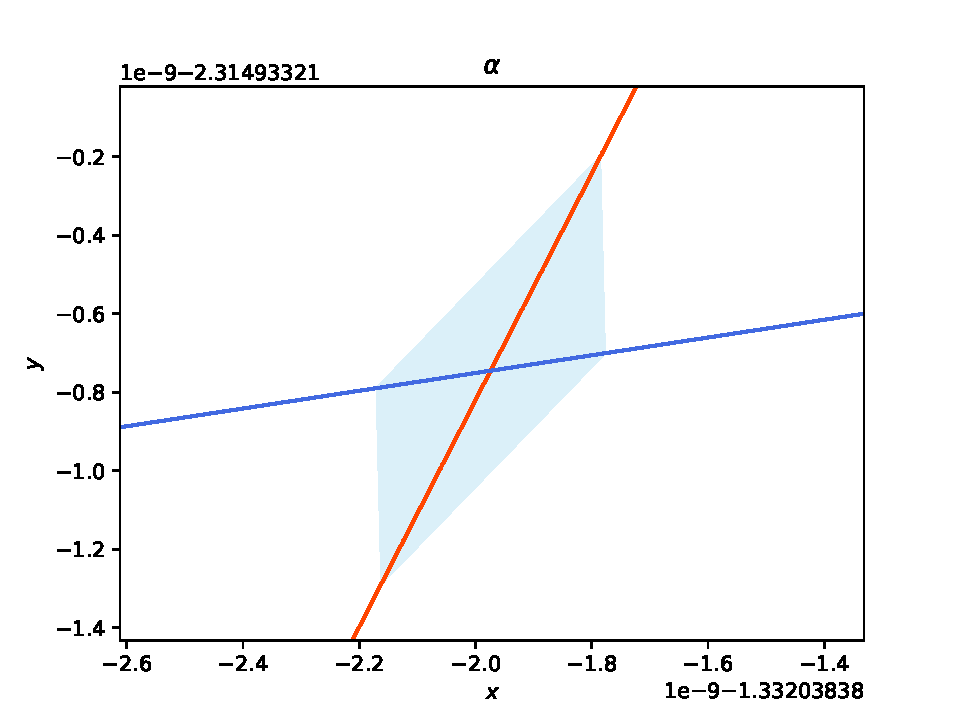
\includegraphics[width=50mm]{alpha}
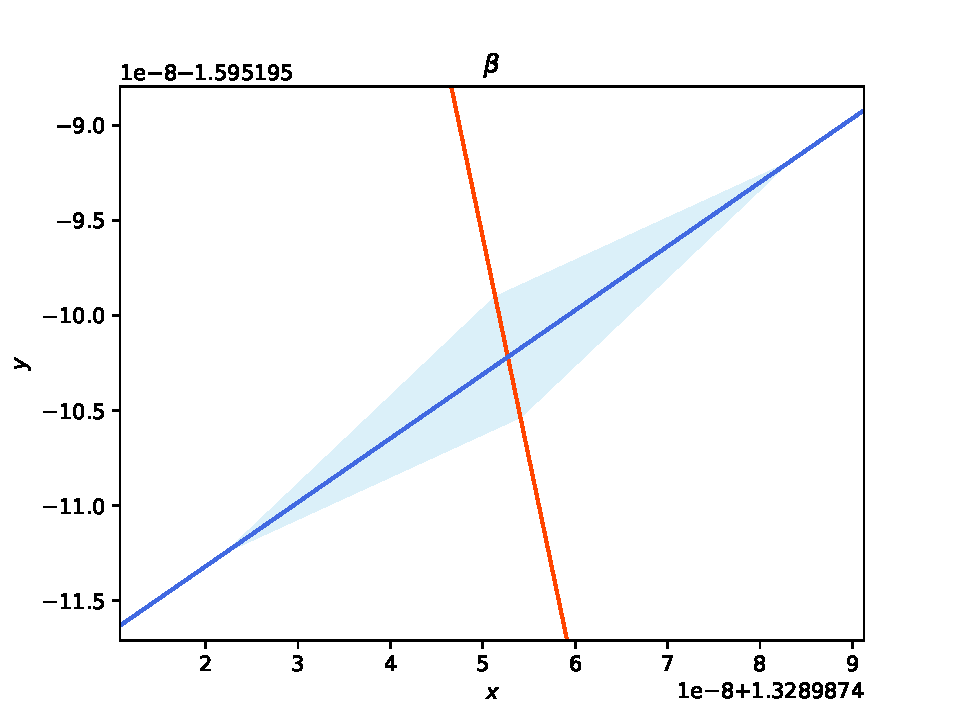
\includegraphics[width=50mm]{beta}
\caption{Intervalos de intersecciones entre las variedades estable e inestable del mapeo de Hénon.} 
\label{matriz_cortes}
\end{figure}
\end{frame}


\begin{frame}{Exponencial}
\begin{figure}[H]
\centering
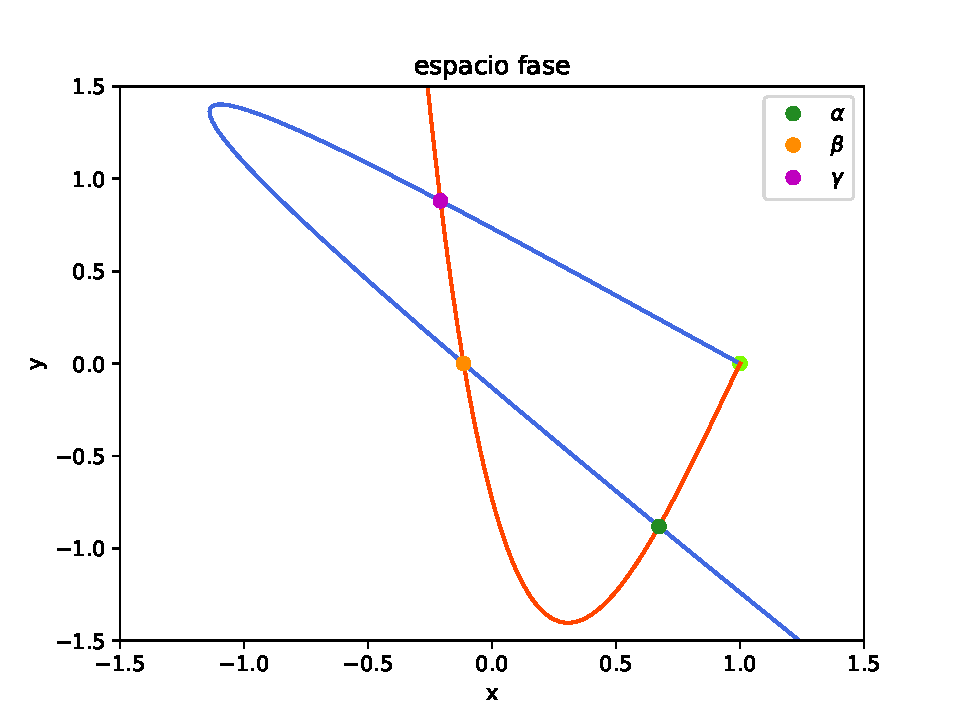
\includegraphics[scale=0.5]{cruces_jung1}
\caption{Intersecciones en el mapeo exponencial con $a=5.7$, con una tolerancia de $10^{-6}$.}
\label{jung_cortes}
\end{figure}
\end{frame}

\begin{frame}
\begin{figure}
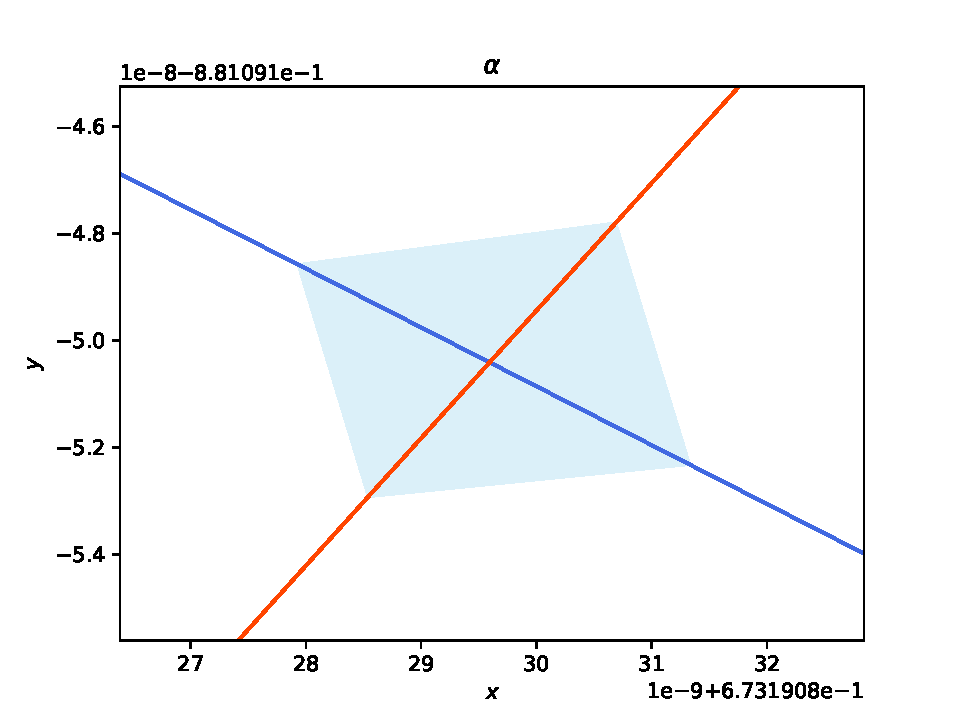
\includegraphics[width=40mm]{cruce_a}
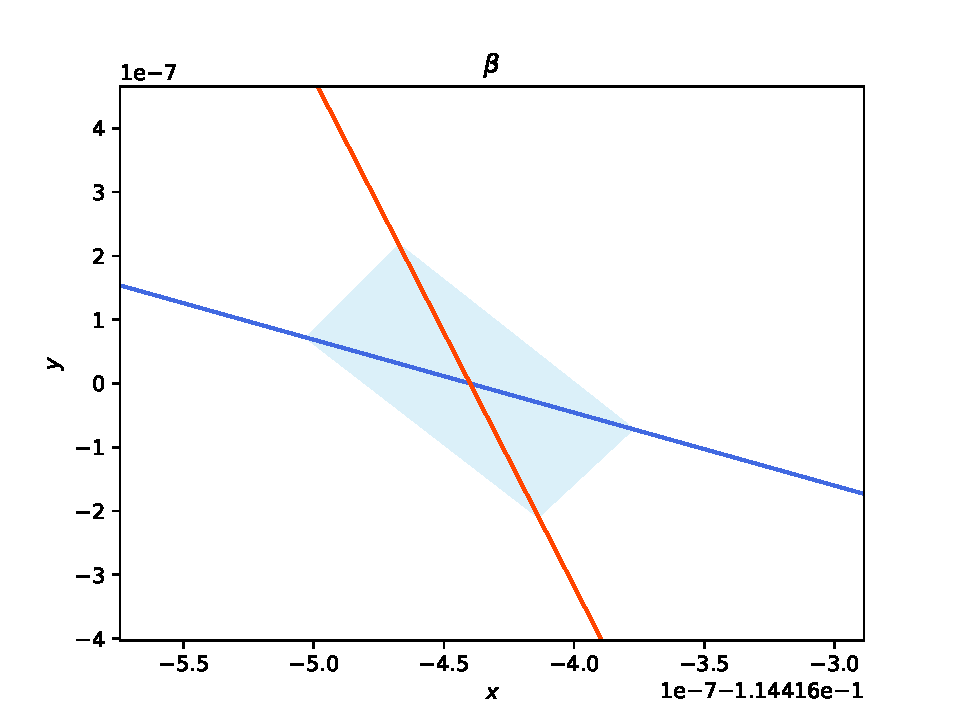
\includegraphics[width=40mm]{cruce_b}
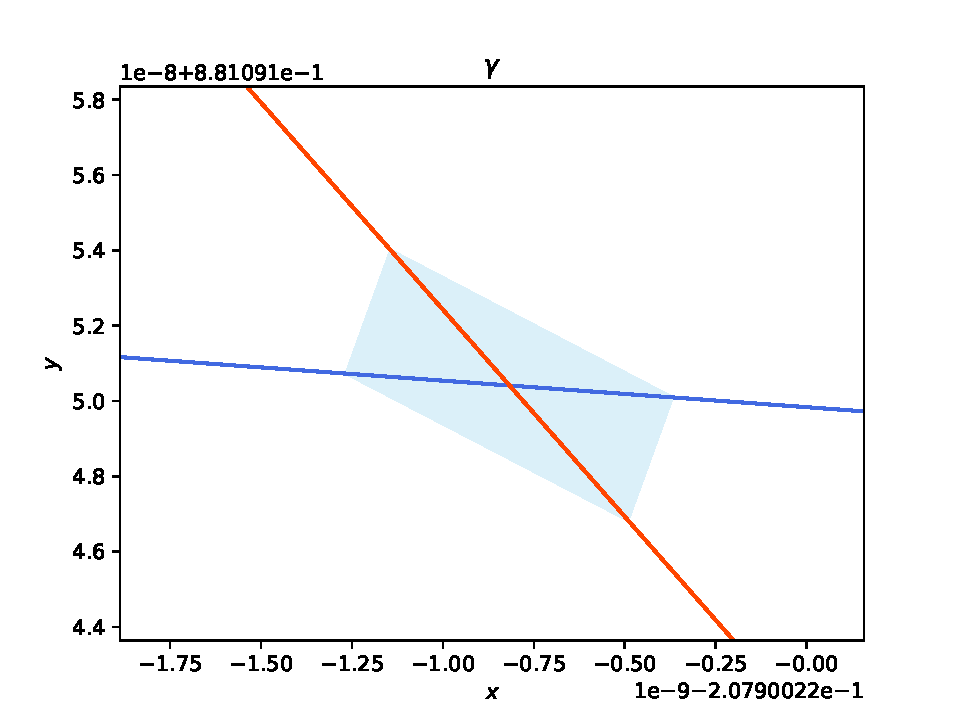
\includegraphics[width=40mm]{cruce_c}
\caption{Intervalo de intersección de las variedades estable e inestable en el mapeo exponencial.} 
\label{cruces_jung}
\end{figure}
\end{frame}

\begin{frame}{Rect\'angulo fundamental}

\begin{figure}
\centering
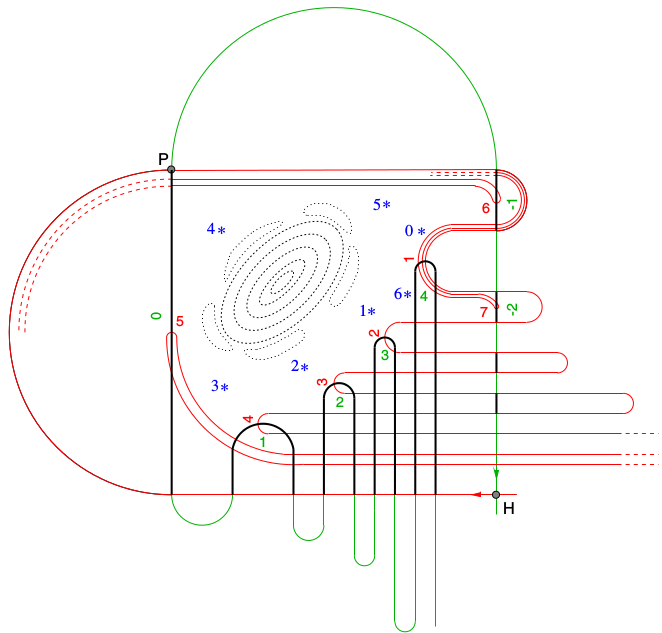
\includegraphics[scale=0.27]{herradura}
\caption{Diagrama ilustrativo de la topología de una herradura en un sistema Hamiltoniano de dos dimensiones.\cite{Merlo} }
%Tomada de \cite{Merlo}, pp.8.} H denota el punto fijo hiperbólico y P la primera intersección. Los tentáculos de la variedad estable son enfatizados con color negro. Tomada de \cite{Merlo}, pp.8.}
\label{herradura}
\end{figure}

\end{frame}
%-----------------------------------------------------------------------------
\begin{frame}
Reescribiendo la ecuación de invariancia \eqref{Ecua de invariancia} para el caso de la variedad estable, se obtiene:
\begin{eqnarray}
f_{a,b}^{-1}(W_{0}^{s}(t))=W_{0}^{s}(\lambda^{m}t).
\label{InvarianciaEstable1}
\end{eqnarray}

Aplicando el mapeo de Hénon  \eqref{Henon} a la ecuación \eqref{InvarianciaEstable1} resulta
\begin{eqnarray}
W_{0}^{s}(t)=f_{a,b}(W_{0}^{s}(\lambda^{m}t)),
\label{InvarianciaEstable2}
\end{eqnarray}
que se reescribe como \eqref{InvarianciaEstable2}, 
\begin{eqnarray}
W_{0}^{s}\left(\frac{t}{\lambda^{m}}\right)=f_{a,b}(W_{0}^{s}(t)).
\label{InvarianciaEstable3}
\end{eqnarray}

Como $\vert \lambda^{m} \vert < 1 $ la ecuación \eqref{InvarianciaEstable3} muestra que aplicar el mapeo es análogo a tener la variedad estable evaluada en un valor mayor del parámetro, puesto que $1/\lambda^{m}>1$. 
\end{frame}


%----------------------------------------------------------------------------
\begin{frame}
\begin{figure}[H]
\centering
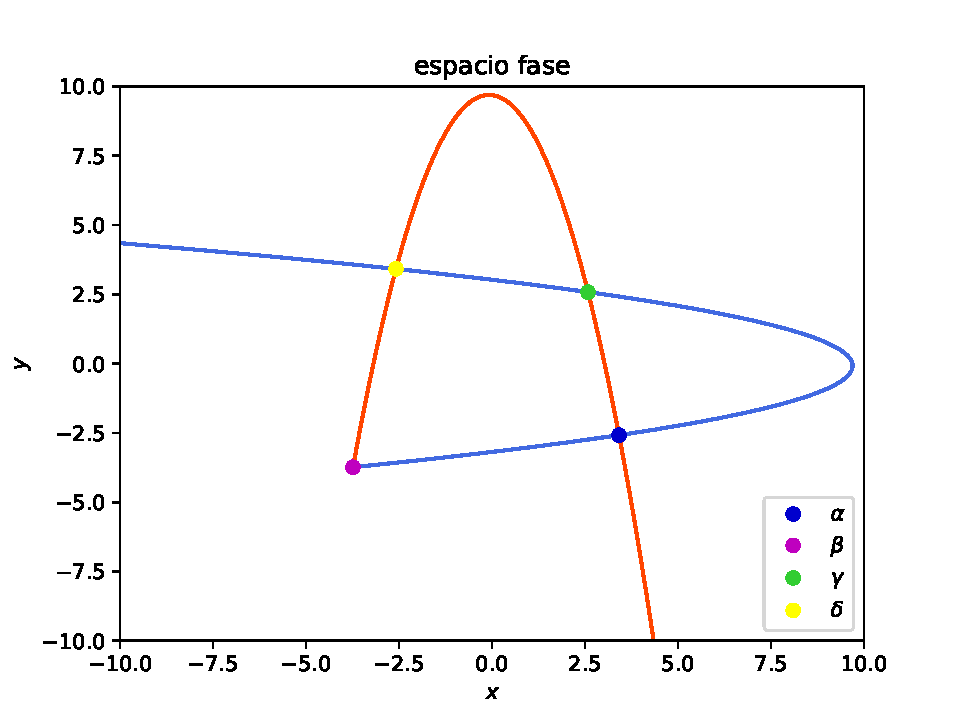
\includegraphics[scale=0.5]{rectangulo_fundamental}
\caption{Variedades estable e inestable de orden 250, para el mapeo de Hénon con $a=6.5,b=1.$, en el intervalo $t=[0.,100.]$. El punto $\omega$ denota el punto fijo mientras que $\alpha, \beta, \gamma$ son las primeras intersecciones de las variedades.}
\label{rectangulo0}
\end{figure}
\end{frame}
%----------------------------------------------------------------------------
\begin{frame}
\begin{figure}[H]
\centering
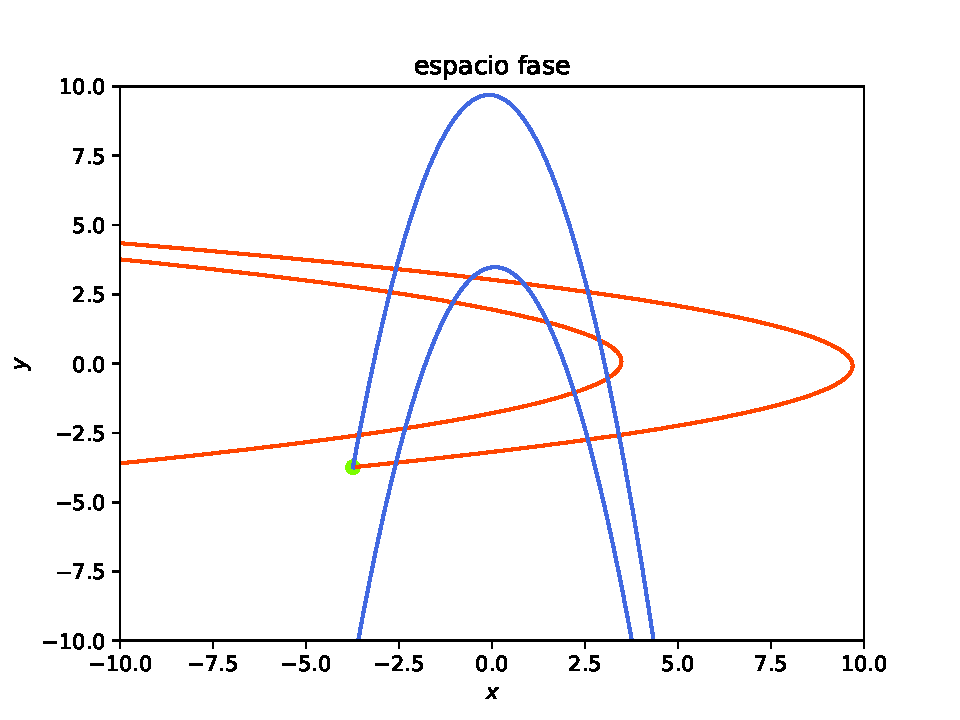
\includegraphics[scale=0.5]{rectangulo1.pdf}
\caption{Primera aplicación del mapeo a los polinomios de orden 250, $t=[0,100]$.}
\label{Rectangulo1}
\end{figure}
\end{frame}
%--------------------------------------------------------------------------
\begin{frame}
Para saber cuál es este error se usó la ecuación \eqref{InvarianciaEstable3},
\begin{eqnarray}
E_{1}(t)=\bigg\| W_{0}^{s}\left(\frac{t}{\lambda^{m}}\right)-f_{a,b}(W_{0}^{s}(t))\bigg\|_{\infty},
\label{error-1aplicacion}
\end{eqnarray}
generalizando obtenemos
\begin{eqnarray}
E_{n}(t)=\bigg\| (f_{k})^{n}\left(W_{0}^{s}\left(\frac{t}{\lambda^{m}}\right)\right)- (f_{k})^{n-1}(W_{0}^{s}(t)))\bigg\|_{\infty}.
\label{error-n-aplicacion}
\end{eqnarray}
\end{frame}
%----------------------------------------------------------------------------
\begin{frame}
\begin{figure}[h!]
\centering
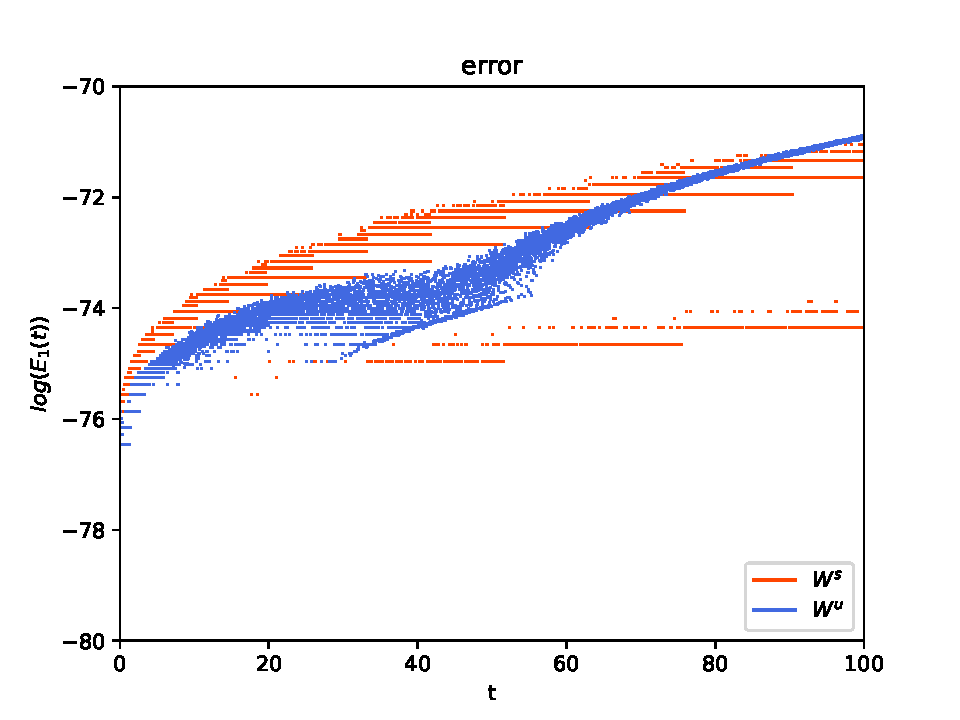
\includegraphics[scale=0.6]{error1ite.pdf}
\caption{Error en el polinomio que resulta de aplicar el mapeo a la parametrización de orden 250.}
\label{error-1iteracion}
\end{figure}
\end{frame}
%-------------------------------------------------------------------------
\begin{frame}
La segunda aplicación del mapeo a los polinomios, $(W_{x2}^{s},W_{y2}^{s})=f_{a,b}(W_{x1}^{s},W_{y1}^{s})$
\begin{figure}[h!]
\centering
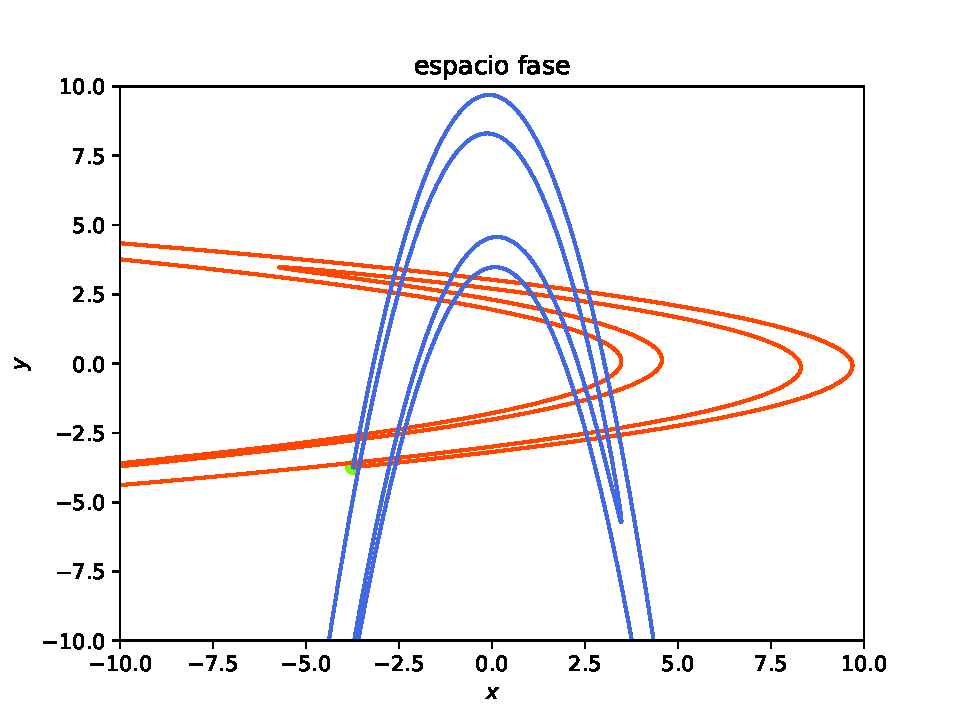
\includegraphics[scale=0.6]{rectangulo2.pdf}
\caption{Segunda aplicación del mapeo a los polinomios de orden 250.}
\label{Rectangulo2}
\end{figure}

\end{frame}
%-----------------------------------------------------------------------
\begin{frame}
La tercera aplicaci\'on
\begin{figure}[h!]
\centering
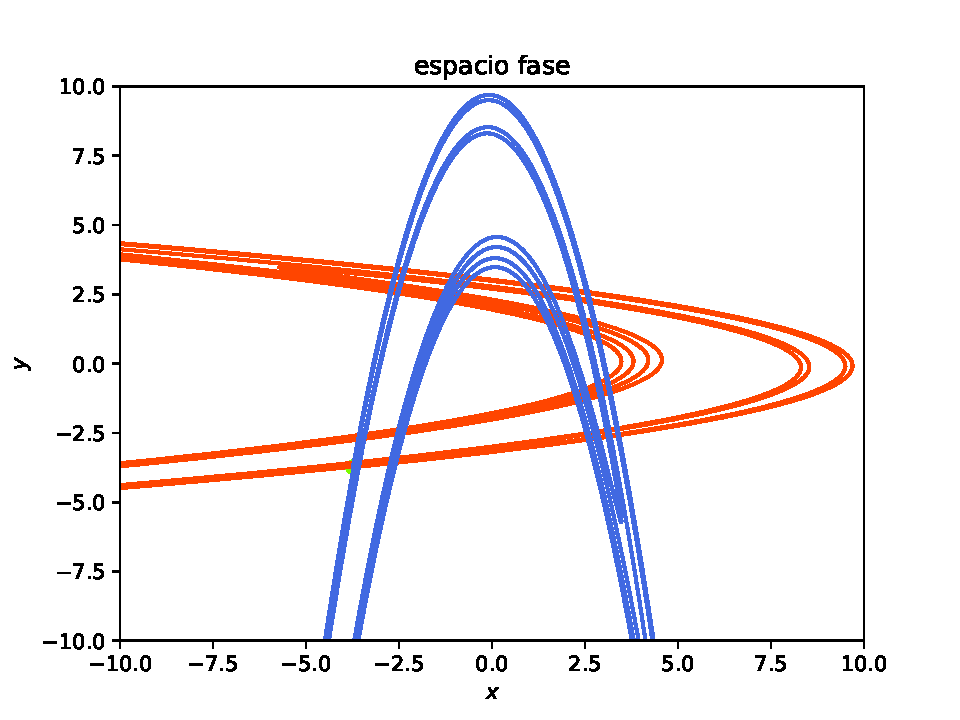
\includegraphics[scale=0.6]{rectangulo3.pdf}
\caption{Tercer aplicación del mapeo a los polinomios de orden 250.}
\label{Rectangulo3}
\end{figure}
\end{frame}
%------------------------------------------------------------------------
\begin{frame}
\begin{figure}[h!]
\centering
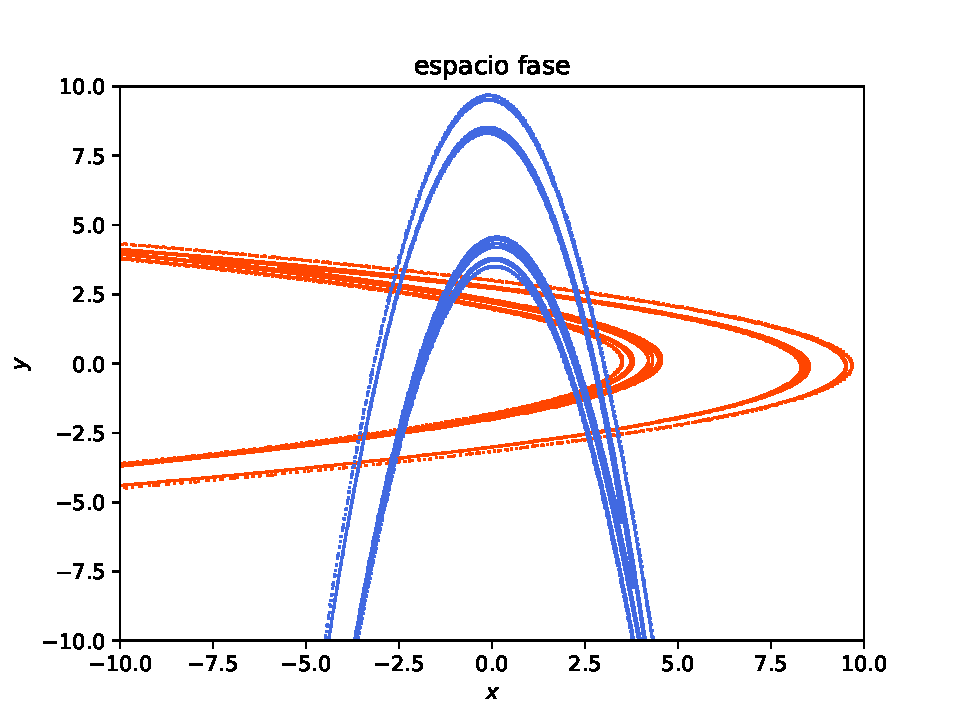
\includegraphics[scale=0.6]{rectangulo4.pdf}
\caption{Cuarta aplicación del mapeo a los polinomios de orden 250.}.
\label{Rectangulo4}
\end{figure}
\end{frame}
%---------------------------------------------------------------------
\begin{frame}
\begin{figure}[H]
\centering
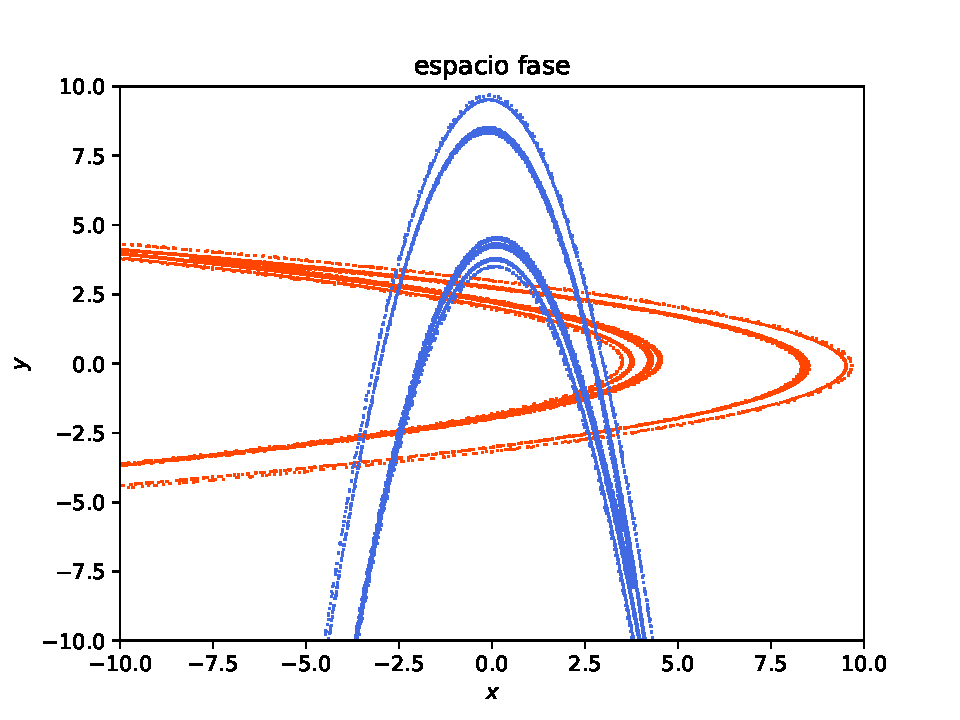
\includegraphics[scale=0.6]{rectangulo5.pdf}
\caption{Quinta aplicación del mapeo a los polinomios de orden 250.}.
\label{Rectangulo5}
\end{figure}
\end{frame}
%------------------------------------------------------------------------------
\begin{frame}{Conclusiones y perspectivas}
\justifying
\begin{itemize}
    \item El método es eficiente para calcular variedades estables e inestables en comparación con los métodos iterativos.
    \item Se puede estudiar más sobre el comportamiento de las variedades.
    \item Es posible calcular puntos homoclínicos y heteroclínicos.
    \item Mediante la iteración de la parametrización bajo el mapeo es posible obtener más sobre las variedades.
    \item Generalizar el método para otro tipo de sistemas.
    \item Utilizar cómputo validado.
\end{itemize}


\end{frame}

\begin{frame}[allowframebreaks]
  \frametitle{Bibliografía}
  
  \nocite{Mireles, Mireles2,Haro,Meyer, gerald,Meiss, Chang, Merlo,Juergen, Tomoki, Jung,Jung2, Seligman, Ott,gold, arnold,arn,hale, ver, devaney,devaney2,marion, ramon, interval,validated, static,root,Friedberg, Mateo,book:Calvin,Numerics,Ying}
  
  \bibliographystyle{plain}
  \bibliography{referencias}
\end{frame}


\end{document}